\documentclass[../../thesis.tex]{subfiles}

\begin{document}

In this section we present the results from both the experiments on stage 1 and 2, while addressing the research questions. \newline

To summarize NC-VQVAE is able to capture the conditional distribution of the data better than naive VQVAE for a wide variety of datasets. For datasets with few training samples, our model can be prone to overfitting. We see our model as a step in the right direction, but further development is needed to ensure better intraclass diversity, possibly through a more refined sampling procedure. \newline

Key takeaways: We are able to simultaneously reconstruct well and significantly improve downstream classification accuracy, which is very interesting from a representation learning perspective. We improve both IS, FID and CAS for most datasets, indicating that the conditional distribution is better captured, as well as the synthetic data being closer to the ground truth. Additionally we see some differences in Barlow Twins and VIbCReg when it comes to sample diversity.\newline

NC-VQVAE is better able to mimic the training data. When data is abundant, then our model better captures the entire distribution, while covering \newline

Some of the issues of TimeVQVAE are still highly relevant, such as the difficulty in modelling data with sharp differences in modularity, such as TwoPatterns and ElectricDevices.

\section{Stage 1}
In this section we present the results of the tokenization model, in particular the reconstruction loss and the downstream classification accuracy. We address research question 1 and 2, if the proposed NC-VQVAE is able to reconstruct on par with the naive VQVAE and if the learned latent representations are more expressive, in the sense that they simultaneously improve the downstream classification accuracy. We see that some configuration of NC-VQVAE is the top performer on the majority of datasets for both metrics, and provides significant increase in probe accuracy. 

\subsection{Reconstruction}

We present top 1 and mean reconstruction loss across the four runs in table \ref{tab:best_recons} and table \ref{tab:mean_recons} respectively.

\begin{table}[H]
    \centering
    \title{Mean validation reconstruction error}
    \begin{adjustbox}{width=\textwidth}
    \begin{tabular}{lc|c|c|c|c|c|c} % 8 cols, 1 for dataset, 7 for val_recons across models (7 models)
        \toprule
        \multirow{3}{*}{\textbf{Dataset}} & \multicolumn{1}{c}{\textbf{Baseline}} & \multicolumn{6}{c}{\textbf{SSL Method}} \\
                                         \cmidrule(lr){3-8}
                                          & \multicolumn{1}{c}{Regular}           & \multicolumn{3}{c}{Barlow Twins}    &  \multicolumn{3}{c}{VIbCReg} \\
                                                                                   \cmidrule(lr){3-5}                    \cmidrule(lr){6-8}
                                          &   None                                & Warp  & Slice & Gauss               & Warp & Slice & Gauss \\
                            
        \midrule
        FordA                   & 0.217 & 0.127 & 0.134 & \textbf{0.108} & 0.173 & 0.169 & 0.203 \\
        ElectricDevices         & \textbf{0.041} & 0.067 & 0.044 & 0.049 & 0.105 & 0.042 & 0.049 \\
        StarLightCurves         & \textbf{0.032} & 0.042 & 0.069 & 0.071 & 0.052 & 0.050 & 0.068 \\
        Wafer                   & 0.044 & 0.037 & 0.048 & 0.049 & \textbf{0.035} & 0.042 & 0.039 \\
        ECG5000                 & \textbf{0.048} & 0.083 & 0.170 & 0.104 & 0.093 & 0.205 & 0.064 \\
        TwoPatterns             & 0.197 & 0.201 & \textbf{0.184} & 0.230 & 0.214 & 0.186 & 0.207 \\
        UWaveGestureLibraryAll  & 0.190 & \textbf{0.172} & 0.190 & 0.245 & 0.189 & 0.178 & 0.237 \\
        FordB                   & 0.150 & 0.115 & 0.122 & 0.123 & \textbf{0.114} & 0.121 & 0.142 \\
        ShapesAll               & \textbf{0.045} & 0.056 & 0.066 & 0.102 & 0.064 & 0.069 & 0.073 \\
        SonyAIBORobotSurface1   & 0.402 & 0.509 & 0.494 & 0.491 & \textbf{0.360} & 0.363 & 0.418 \\
        SonyAIBORobotSurface2   & 0.623 & 0.622 & 0.618 & 0.640 & 0.487 & \textbf{0.454} & 0.589 \\
        Symbols                 & 0.110 & 0.143 & 0.134 & 0.173 & 0.078 & \textbf{0.067} & 0.105 \\
        Mallat                  & 0.066 & 0.081 & 0.091 & 0.096 & 0.066 & 0.067 & \textbf{0.060} \\
        \bottomrule
    \end{tabular}
    \end{adjustbox}
    \caption{Mean validation reconstruction error across all 13 datasets. Results are averaged over four runs.}
    \label{tab:mean_recons}
\end{table}

\begin{table}[H]
    \centering
    \title{Top 1 validation reconstruction error}
    \begin{adjustbox}{width=\textwidth}
    \begin{tabular}{lc|c|c|c|c|c|c} % 8 cols, 1 for dataset, 7 for val_recons across models (7 models)
        \toprule
        \multirow{3}{*}{\textbf{Dataset}} & \multicolumn{1}{c}{\textbf{Baseline}} & \multicolumn{6}{c}{\textbf{SSL Method}} \\
                                         \cmidrule(lr){3-8}
                                          & \multicolumn{1}{c}{Regular}           & \multicolumn{3}{c}{Barlow Twins}    &  \multicolumn{3}{c}{VIbCReg} \\
                                                                                   \cmidrule(lr){3-5}                    \cmidrule(lr){6-8}
                                          &   None                                & Warp  & Slice & Gauss               & Warp & Slice & Gauss \\
                            
        \midrule
        FordA                   & 0.158 & 0.108 & 0.111 & \textbf{0.087} & 0.130 & 0.134 & 0.113 \\
        ElectricDevices         & 0.036 & 0.060 & 0.034 & 0.043 & 0.092 & \textbf{0.031} & 0.045 \\
        StarLightCurves         & \textbf{0.026} & 0.037 & 0.057 & 0.055 & 0.043 & 0.048 & 0.065 \\
        Wafer                   & 0.038 & 0.031 & 0.045 & 0.043 & \textbf{0.027} & 0.031 & 0.038 \\
        ECG5000                 & \textbf{0.044} & 0.069 & 0.156 & 0.084 & 0.080 & 0.181 & 0.056 \\
        TwoPatterns             & 0.181 & 0.184 & \textbf{0.169} & 0.208 & 0.200 & 0.172 & 0.185 \\
        UWaveGestureLibraryAll  & 0.159 & \textbf{0.145} & 0.167 & 0.201 & 0.155 & 0.169 & 0.233 \\
        FordB                   & 0.117 & 0.094 & 0.090 & 0.103 & \textbf{0.082} & 0.094 & 0.102 \\
        ShapesAll               & \textbf{0.035} & 0.043 & 0.046 & 0.092 & 0.061 & 0.063 & 0.067 \\
        SonyAIBORobotSurface1   & 0.381 & 0.473 & 0.472 & 0.465 & 0.329 & \textbf{0.328} & 0.408 \\
        SonyAIBORobotSurface2   & 0.513 & 0.577 & 0.536 & 0.588 & 0.444 & \textbf{0.414} & 0.470 \\
        Symbols                 & 0.088 & 0.111 & 0.122 & 0.150 & 0.062 & \textbf{0.059} & 0.090 \\
        Mallat                  & 0.061 & 0.075 & 0.076 & 0.088 & 0.059 & 0.059 & \textbf{0.057} \\

  
        \bottomrule
    \end{tabular}
    \end{adjustbox}
    \caption{Top 1 validation reconstruction error across all 13 datasets. Lowest value of the four runs for each model is selected.}
    \label{tab:best_recons}
\end{table}

We observe that NC-VQVAE reconstructs on par with the baseline model, and that some configuration outperforms the naive VQVAE on mean reconstruction loss for 9 out of 13 datasets.\newline

In figure \ref{fig:Mean_val_recons} observe that the difference in reconstruction loss is small for most datasets, both across SSL methods and augmentations. Nevertheless we observe that VIbCReg generally performs slightly better than Barlow Twins, except for FordA. Additionally the use of gaussian augmentation introduces less of a regularizing effect compared to the two other sets of augmentations, with the exception of Slice and Shuffle on ECG5000. These results show that the introduction of a non contrastive loss does not hurt the reconstruction capabilities, compared to naive VQVAE. \newline

\begin{figure}[h]
    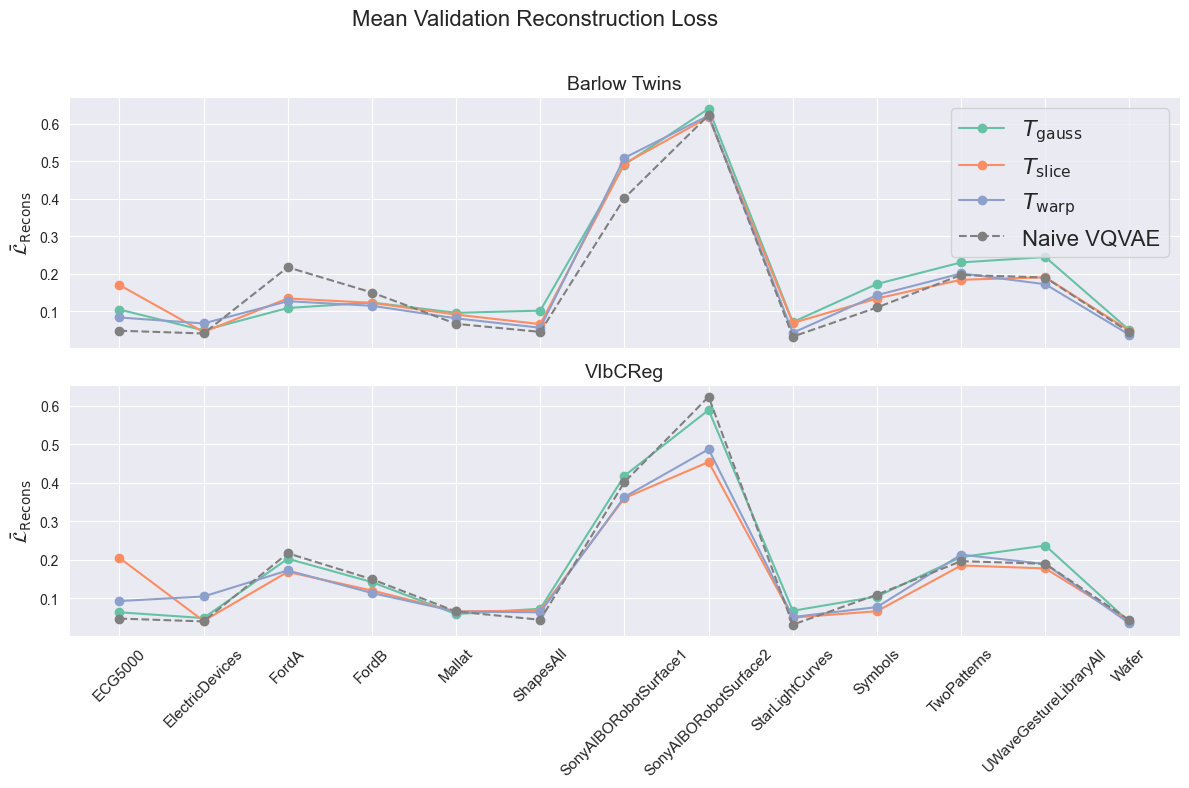
\includegraphics[scale=0.4]{Mean_val_recons.png}
    \centering  
    \caption{Mean validation reconstruction loss for the two models, compared to naive VQVAE}
    \label{fig:Mean_val_recons}
\end{figure}

Regarding the effect of by the reconstruction loss of augmented branch on validation reconstruction, a small initial experiment was conducted. The results show that the validation reconstruction loss was quite robust to the particular value of augmentation reconstruction weight, indicating a minor role played, as seen in Figure \ref{fig:ReconsWeight_warp} and \ref{fig:ReconsWeight_slice}.\newline

By investigating the development of the validation reconstruction loss during training, we have observed that right configuration for NC-VQVAE can act as a regularizer. In Figure \ref{fig:FordA_val_recons} we see the development on FordA. 

\begin{figure}[h]
    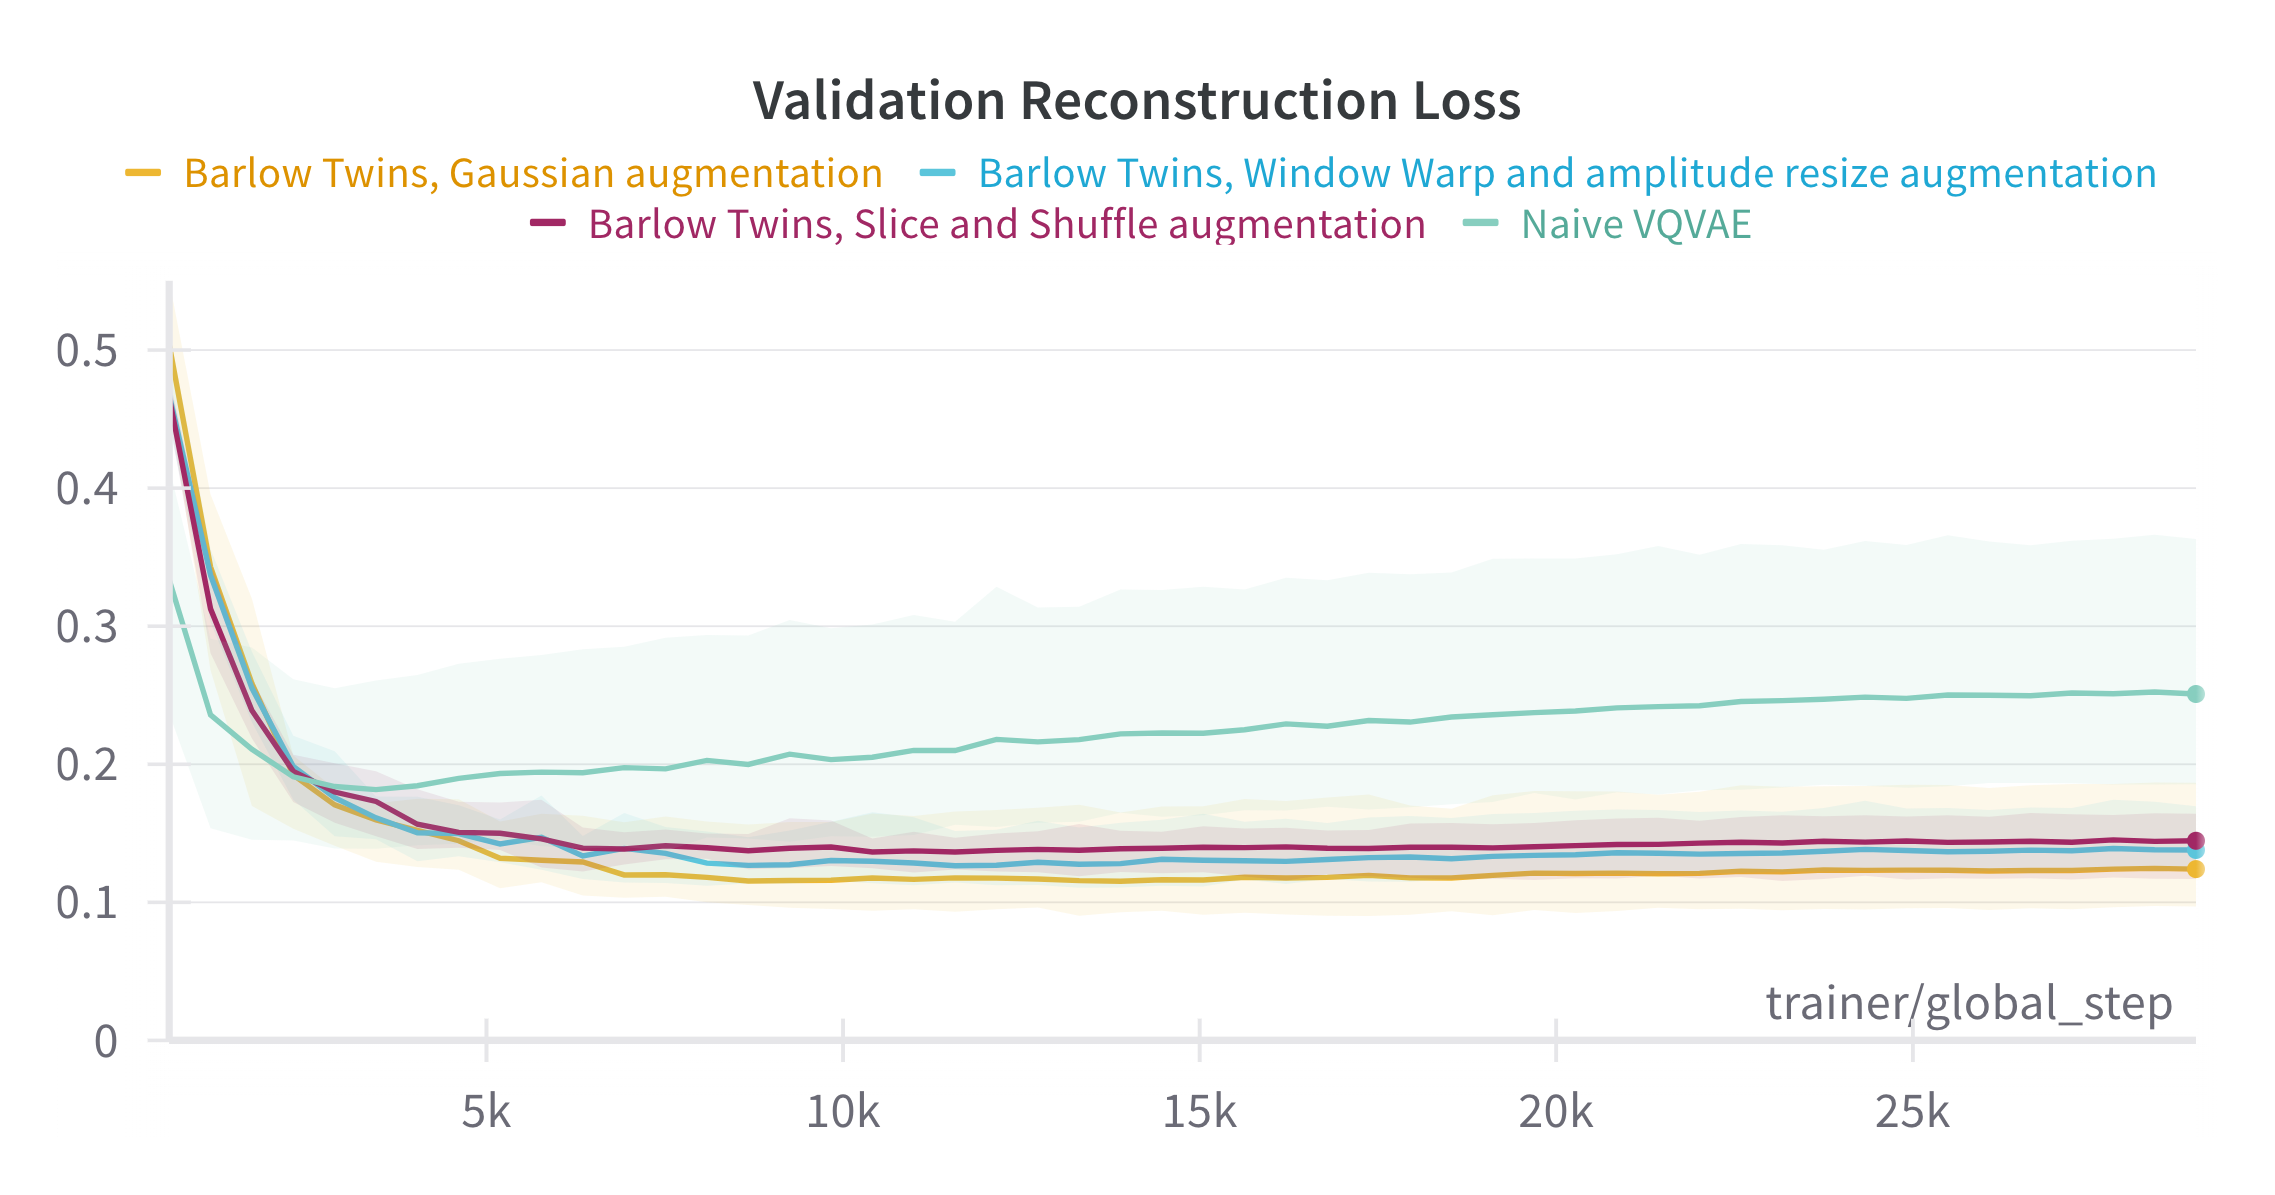
\includegraphics[scale=0.10]{FordA_val_recons.png}
    \centering  
    \caption{Development of the validation reconstruction loss for Barlow Twins and naive VQVAE on FordA during training. Averaged across all four runs. }
    \label{fig:FordA_val_recons}
\end{figure}


\subsection{Classification}

We present the mean and max downstream classification accuracy in table \ref{tab:mean_probe} and \ref{tab:best_probe} respectively. 


\begin{table}[h]
    \centering
    \title{Mean linear probe accuracy}
    \begin{adjustbox}{width=\textwidth}
    \begin{tabular}{lcc|cc|cc|cc|cc|cc|cc} % 15 cols, 1 for dataset, 14 for svm/knn across models (7 models)
        \toprule
        \multirow{4}{*}{\textbf{Dataset}} & \multicolumn{2}{c}{\textbf{Baseline}} & \multicolumn{12}{c}{\textbf{SSL Method}} \\
                                            \cmidrule(lr){2-3} \cmidrule(lr){4-15}
                                          & \multicolumn{2}{c}{Regular}           & \multicolumn{6}{c}{Barlow Twins}                                                 &  \multicolumn{6}{c}{VIbCReg} \\
                                          \cmidrule(lr){2-3} \cmidrule(lr){4-9} \cmidrule(lr){10-15}
                                          &   \multicolumn{2}{c}{None}            & \multicolumn{2}{c}{Warp}  & \multicolumn{2}{c}{Slice} & \multicolumn{2}{c}{Gauss} & \multicolumn{2}{c}{Warp} & \multicolumn{2}{c}{Slice} & \multicolumn{2}{c}{Gauss} \\
                                          \cmidrule(lr){2-3} \cmidrule(lr){4-5} \cmidrule(lr){6-7} \cmidrule(lr){8-9} \cmidrule(lr){10-11} \cmidrule(lr){12-13}\cmidrule(lr){14-15}
                                          & KNN & SVM                               & KNN & SVM                  & KNN & SVM                & KNN & SVM                 & KNN & SVM                 & KNN & SVM                 & KNN & SVM   \\
        \midrule
        FordA                   & 0.70 & 0.74 & 0.83 & 0.84 & \textbf{0.91} & \textbf{0.89} & 0.80 & 0.83 & 0.80 & 0.74 & 0.87 & 0.86 & 0.76 & 0.78 \\
        ElectricDevices         & 0.35 & 0.41 & 0.35 & \textbf{0.44} & 0.38 & 0.41 & \textbf{0.40} & 0.42 & 0.33 & 0.38 & 0.36 & 0.39 & 0.39 & 0.43 \\
        StarLightCurves         & 0.87 & 0.89 & 0.93 & 0.93 & \textbf{0.94} & \textbf{0.94} & 0.88 & 0.88 & 0.92 & \textbf{0.94} & 0.91 & 0.93 & 0.89 & 0.89 \\
        Wafer                   & 0.93 & 0.89 & 0.96 & \textbf{0.94} & 0.96 & \textbf{0.94} & 0.96 & 0.93 & \textbf{0.97} & 0.94 & 0.96 & 0.92 & \textbf{0.97} & 0.92 \\
        ECG5000                 & 0.80 & 0.83 & 0.85 & 0.81 & \textbf{0.88} & 0.84 & 0.86 & \textbf{0.84} & 0.86 & 0.82 & \textbf{0.88} & \textbf{0.84} & 0.84 & 0.82 \\
        TwoPatterns             & 0.34 & 0.53 & \textbf{0.69} &\textbf{ 0.91} & 0.66 & 0.82 & 0.47 & 0.71 & 0.64 & 0.90 & 0.68 & 0.80 & 0.55 & 0.72 \\
        UWaveGestureLibraryAll  & 0.31 & 0.40 & \textbf{0.62} & 0.70 & 0.56 & 0.63 & 0.40 & 0.54 & \textbf{0.62} & \textbf{0.73} & 0.55 & 0.66 & 0.44 & 0.55 \\
        FordB                   & 0.58 & 0.60 & 0.64 & 0.67 & 0.74 & 0.76 & 0.64 & 0.68 & 0.63 & 0.64 & 0.70 & 0.70 & 0.61 & 0.64\\
        ShapesAll               & 0.29 & 0.30 & 0.49 & 0.55 & 0.53 & \textbf{0.60} & 0.40 & 0.48 & 0.48 & 0.56 &\textbf{ 0.54} & \textbf{0.60} & 0.40 & 0.46 \\
        SonyAIBORobotSurface1   & 0.56 & 0.68 & 0.54 & 0.70 & \textbf{0.61} & \textbf{0.74} & 0.53 & 0.70 & 0.48 & \textbf{0.74} & 0.58 & 0.71 & 0.54 & 0.69 \\
        SonyAIBORobotSurface2   & \textbf{0.81} & \textbf{0.86} & 0.77 & 0.79 & 0.80 & 0.80 & 0.80 & 0.81 & 0.77 & 0.85 & 0.80 & 0.85 & 0.80 & 0.85  \\
        Symbols                 & 0.50 & 0.60 & \textbf{0.59} & 0.60 & 0.50 & \textbf{0.66} & \textbf{0.59} & \textbf{0.66} & 0.45 & 0.61 & 0.42 & 0.62 & 0.43 & 0.63 \\
        Mallat                  & 0.63 & 0.77 & 0.72 & 0.81 & 0.76 & 0.83 & 0.68 & 0.78 & \textbf{0.79} & \textbf{0.87} & 0.77 & 0.85 & 0.69 & \textbf{0.86} \\
        \bottomrule
    \end{tabular}
    \end{adjustbox}
    
    \caption{Summary of mean linear probe accuracy by SSL Method and Augmentation. Average across 4 seeds. Best result for KNN and SVM are highlighted in bold.}
    \label{tab:mean_probe}
\end{table}

\begin{table}[H]
    \centering
    \title{Top 1 linear probe accuracy}
    \begin{adjustbox}{width=\textwidth}
    \begin{tabular}{lcc|cc|cc|cc|cc|cc|cc} % 15 cols, 1 for dataset, 14 for svm/knn across models (7 models)
        \toprule
        \multirow{4}{*}{\textbf{Dataset}} & \multicolumn{2}{c}{\textbf{Baseline}} & \multicolumn{12}{c}{\textbf{SSL Method}} \\
                                            \cmidrule(lr){2-3} \cmidrule(lr){4-15}
                                          & \multicolumn{2}{c}{Regular}           & \multicolumn{6}{c}{Barlow Twins}                                                 &  \multicolumn{6}{c}{VIbCReg} \\
                                          \cmidrule(lr){2-3} \cmidrule(lr){4-9} \cmidrule(lr){10-15}
                                          &   \multicolumn{2}{c}{None}            & \multicolumn{2}{c}{Warp}  & \multicolumn{2}{c}{Slice} & \multicolumn{2}{c}{Gauss} & \multicolumn{2}{c}{Warp} & \multicolumn{2}{c}{Slice} & \multicolumn{2}{c}{Gauss} \\
                                          \cmidrule(lr){2-3} \cmidrule(lr){4-5} \cmidrule(lr){6-7} \cmidrule(lr){8-9} \cmidrule(lr){10-11} \cmidrule(lr){12-13}\cmidrule(lr){14-15}
                                          & KNN & SVM                               & KNN & SVM                  & KNN & SVM                & KNN & SVM                 & KNN & SVM                 & KNN & SVM                 & KNN & SVM   \\
        \midrule
        FordA                   & 0.75 & 0.78 & 0.84 & 0.88 & \textbf{0.93} & \textbf{0.92} & 0.85 & 0.87 & 0.81 & 0.77 & 0.88 & 0.90 & 0.86 & 0.85 \\
        ElectricDevices         & 0.35 & 0.43 & 0.36 & 0.45 & 0.39 & 0.43 & \textbf{0.45} & \textbf{0.46} & 0.34 & 0.42 & 0.39 & 0.42 & 0.42 & 0.45 \\
        StarLightCurves         & 0.89 & 0.91 & 0.94 & 0.95 & \textbf{0.96} & \textbf{0.96} & 0.90 & 0.91 & 0.95 & 0.95 & 0.93 & 0.95 & 0.90 & 0.90 \\
        Wafer                   & 0.94 & 0.89 &\textbf{ 0.97} & \textbf{0.95} & \textbf{0.97} & \textbf{0.95} & \textbf{0.97} & 0.93 & \textbf{0.97} & \textbf{0.95} & \textbf{0.97} & \textbf{0.95} & \textbf{0.97} & 0.94 \\
        ECG5000                 & 0.83 & 0.84 & 0.88 & 0.86 & \textbf{0.90} & \textbf{0.88} & \textbf{0.90} & \textbf{0.88} & 0.88 & 0.85 & 0.89 & 0.86 & 0.86 & 0.85 \\
        TwoPatterns             & 0.37 & 0.62 & \textbf{0.75} & \textbf{0.96} & 0.68 & 0.85 & 0.55 & 0.75 & 0.70 & 0.92 & 0.71 & 0.81 & 0.63 & 0.76 \\
        UWaveGestureLibraryAll  & 0.34 & 0.43 & \textbf{0.67} & 0.74 & 0.60 & 0.67 & 0.43 & 0.54 & \textbf{0.67} & \textbf{0.76} & 0.58 & 0.67 & 0.48 & 0.58 \\
        FordB                   & 0.60 & 0.63 & 0.67 & 0.71 & \textbf{0.76} & \textbf{0.80} & 0.69 & 0.74 & 0.67 & 0.65 & 0.74 & 0.77 & 0.63 & 0.68 \\
        ShapesAll               & 0.33 & 0.34 & 0.53 & 0.59 & \textbf{0.59} & \textbf{0.65} & 0.44 & 0.50 & 0.50 & 0.56 & 0.57 & 0.63 & 0.44 & 0.48 \\
        SonyAIBORobotSurface1   & 0.67 & \textbf{0.80} & 0.61 & 0.77 & 0.76 & \textbf{0.80} & 0.60 & 0.74 & 0.51 & 0.79 & 0.63 & 0.75 & 0.63 & 0.75 \\
        SonyAIBORobotSurface2   & \textbf{0.84} & \textbf{0.89} & 0.80 & 0.86 & 0.82 & 0.84 & 0.83 & 0.82 & 0.81 & 0.88 & 0.81 & 0.88 & 0.83 & 0.87 \\
        Symbols                 & 0.56 & 0.66 & 0.65 & 0.69 & 0.55 & 0.73 & \textbf{0.64} & \textbf{0.71} & 0.51 & 0.65 & 0.45 & 0.67 & 0.46 & 0.69 \\
        Mallat                  & 0.54 & 0.88 & 0.57 & 0.87 & 0.74 & 0.89 & 0.66 & 0.80 & 0.74 & \textbf{0.92} & 0.72 & 0.88 & 0.62 & \textbf{0.90} \\


        \bottomrule
    \end{tabular}
    \end{adjustbox}
    
    \caption{Summary of max linear probe accuracy by SSL Method and Augmentation. Maximum value across 4 seeds. Best result for KNN and SVM are highlighted in bold.}
    \label{tab:best_probe}
\end{table}

We observe a significant improvement in probe accuracy with NC-VQVAE, compared to naive VQVAE. Some configuration is best on 12 out of 13 datasets, while the one where our model falls short, the difference is one percent for both SVM and KNN. The largest differences are seen on FordA, FordB, Mallat, ShapesAll, TwoPatterns and UWaveGestureLibraryAll.\newline

In Figure \ref{fig:Mean_probe} we observe that even though the specific choice of augmentation has a large impact, on the majority of datasets, all choices result in significantly improved probe accuracy. We note that both SSL methods produce similar probe accuracies for a given augmentation, highlighting the importance of selecting suitable augmentations. \newline
\begin{figure}[h]
    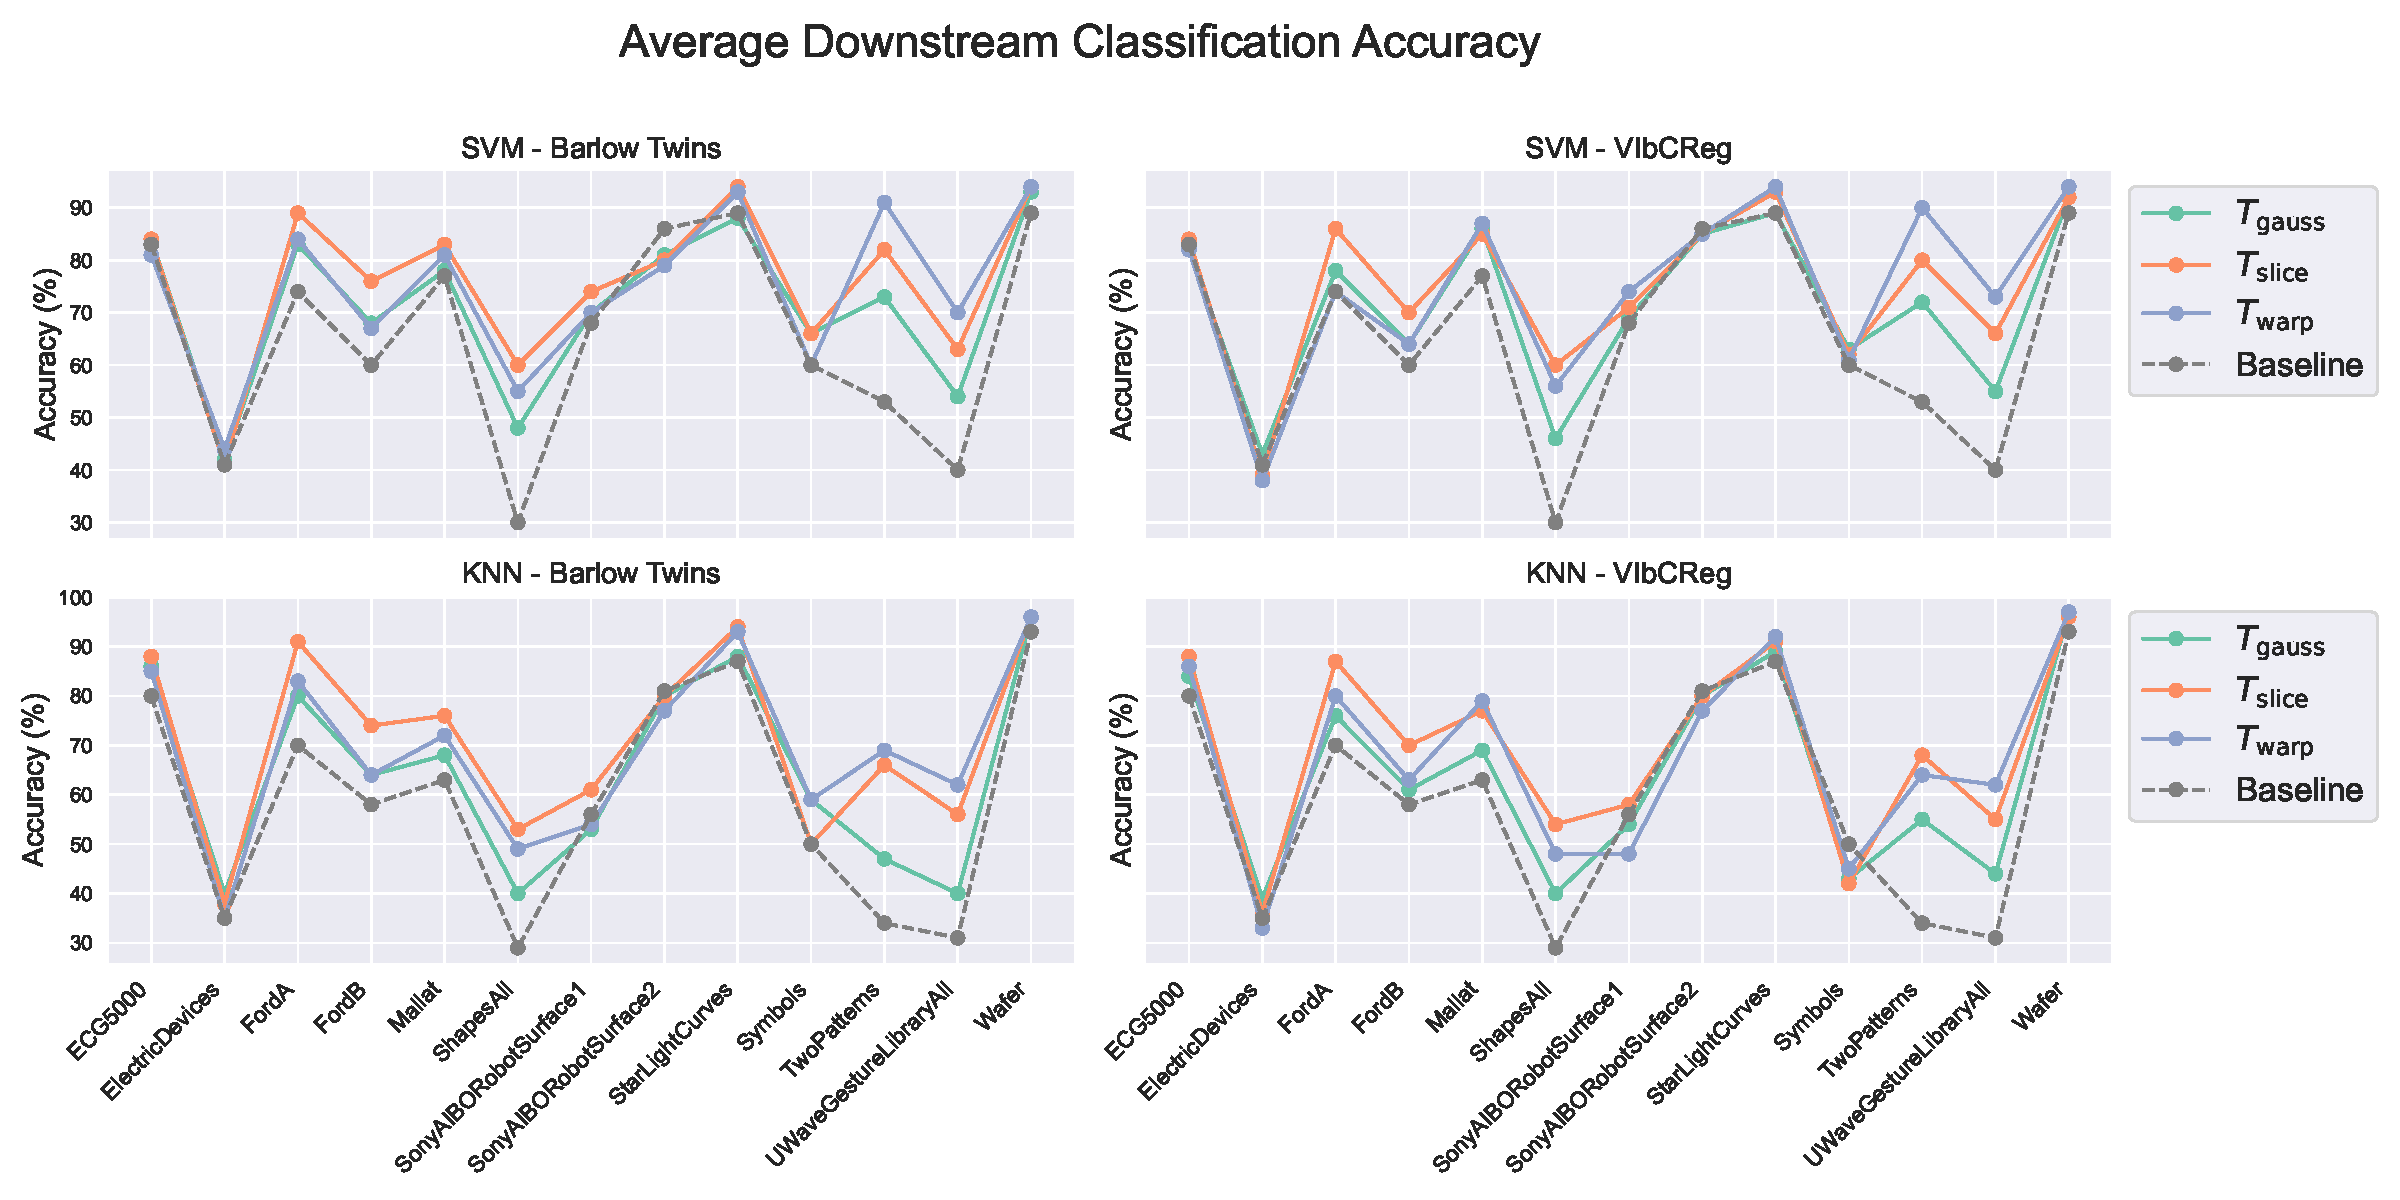
\includegraphics[scale=0.35]{probe_accuracies.pdf}
    \centering  
    \caption{Mean probe accuracies.}
    \label{fig:Mean_probe}
\end{figure}


We observe that Slice and Shuffle, and Window Warp and Amplitude Resize result in the most dramatic increases in accuracy, while Gaussian noise consistently results in less drastic improvement. We hypothesize that, since Slice and Warp often result in augmented views that deviate quite a lot from the original view, the SSL loss pushes the representations in different directions, which again might result in a better utilization of the latent space. In Figure \ref{fig:FordA_TSNE} and \ref{fig:TSNE_TwoPatterns} we see the effect of NC-VQVAE on the discrete latent representations of FordA and TwoPatterns. From these visualizations it is evident that representations learned using NC-VQVAE are more structured than those of the naive VQVAE. Similar samples, typically with the same label, are clustered closer together in latent space. This further indicate that the SSL loss introduces information regarding shape and semantics into the latent representations.\newline

\begin{figure}[h] 
    \centering
    \begin{minipage}[b]{0.32\textwidth}
        \centering
        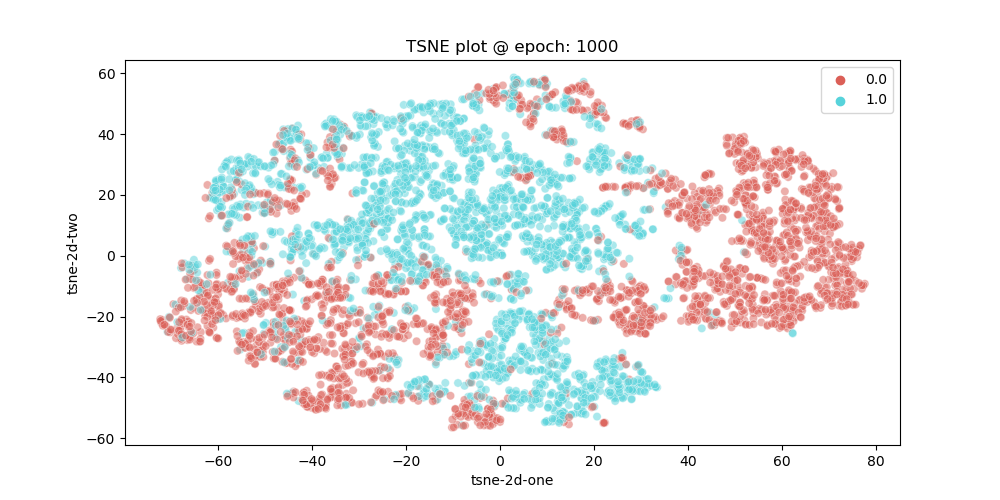
\includegraphics[width=\textwidth]{BT_Slice_FordA_TSNE.png}
    \end{minipage}
    \hfill
    \begin{minipage}[b]{0.32\textwidth}
        \centering
        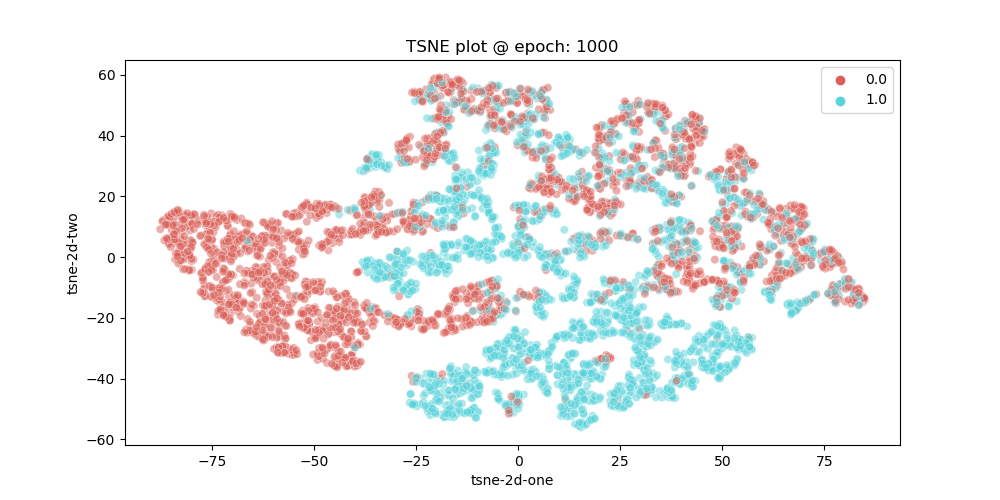
\includegraphics[width=\textwidth]{VIB_Slice_FordA_TSNE.png}
    \end{minipage}
    \hfill
    \begin{minipage}[b]{0.32\textwidth}
        \centering
        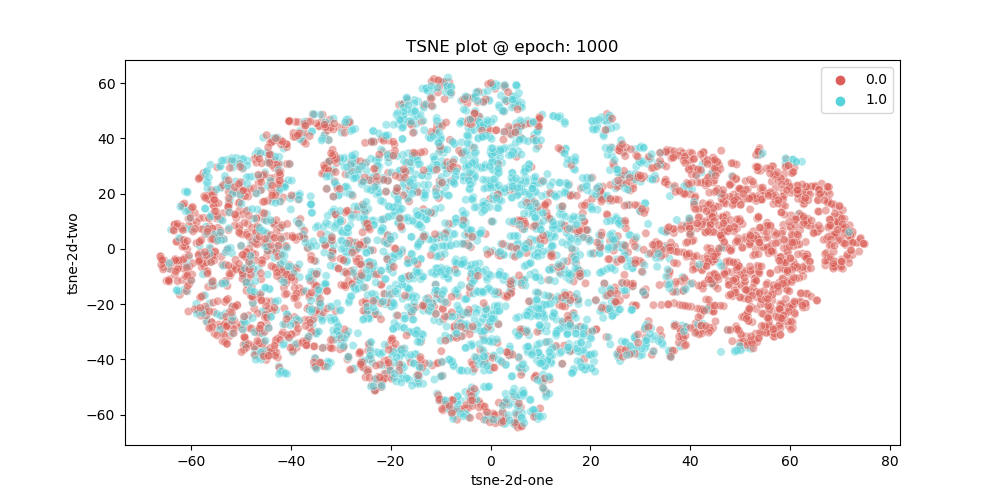
\includegraphics[width=\textwidth]{naive_FordA_TSNE.png}
    \end{minipage}
    \caption{TSNE plots of FordA. Barlow (left) and VIbCReg (center) with Slice and Shuffle, naive VQVAE (right). Best performing model in terms of KNN accuracy is chosen. }
    \label{fig:FordA_TSNE}
\end{figure}


\begin{figure}[h]
    \centering
    \begin{minipage}[b]{0.32\textwidth}
        \centering
        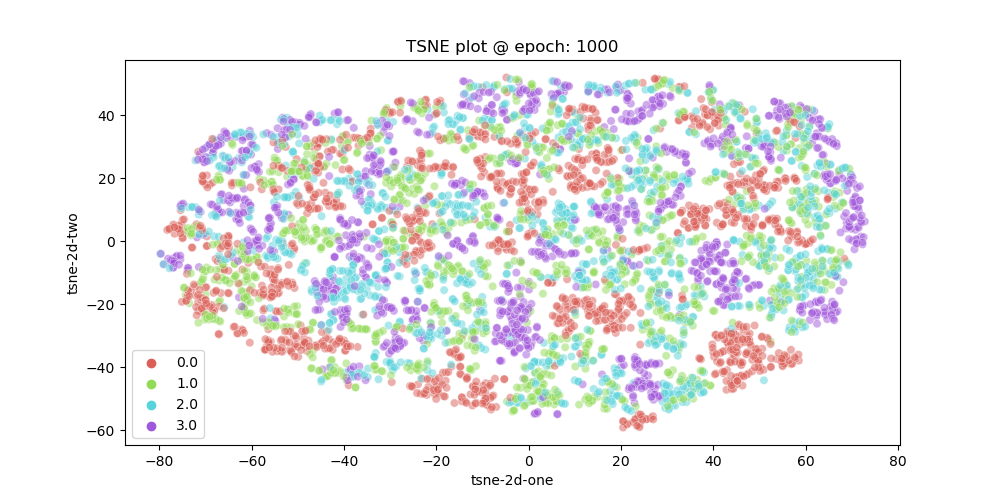
\includegraphics[width=\textwidth]{BT_TwoPatterns_warp_TSNE.png}
    \end{minipage}
    \hfill
    \begin{minipage}[b]{0.32\textwidth}
        \centering
        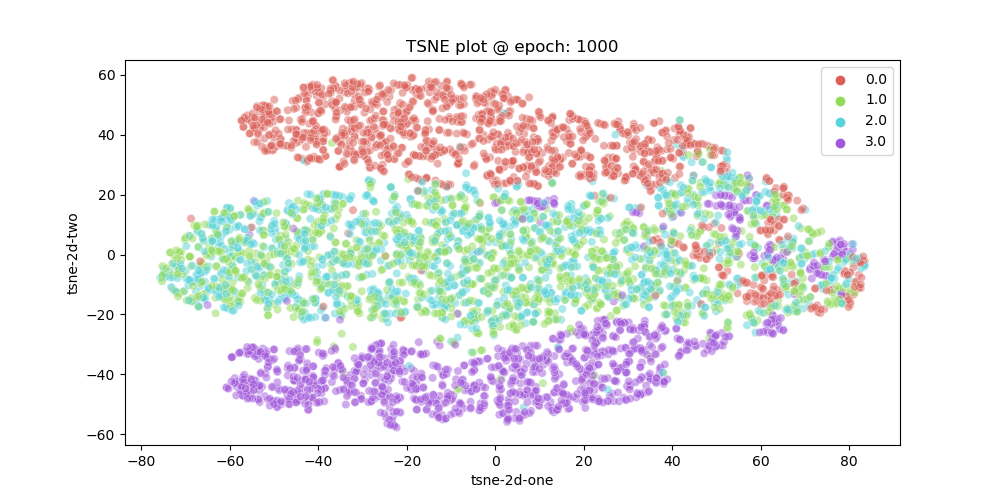
\includegraphics[width=\textwidth]{TSNE_vib_slice_TwoPatterns.png}
    \end{minipage}
    \hfill
    \begin{minipage}[b]{0.32\textwidth}
        \centering
        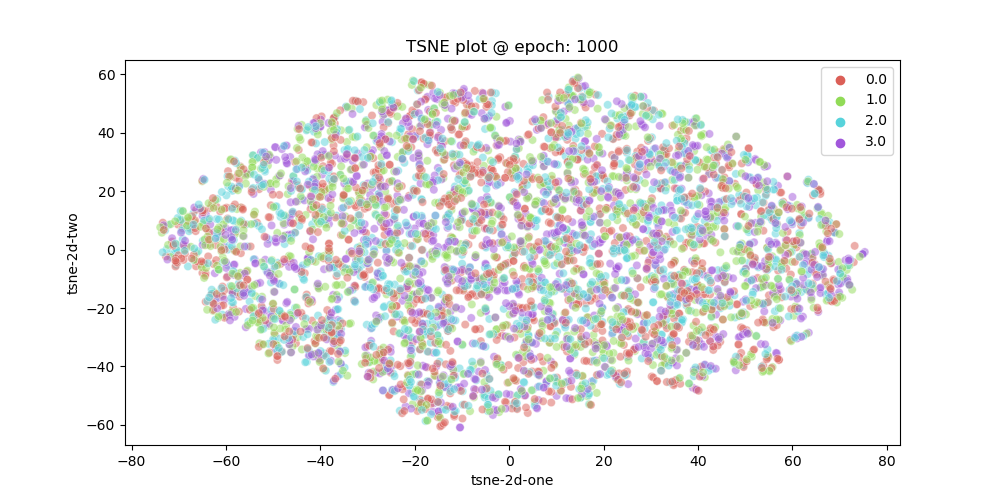
\includegraphics[width=\textwidth]{TSNE_naive_TwoPatterns.png}
    \end{minipage}
    \caption{TSNE plot of discrete latent representations from VIbCReg with Slice and Shuffle (left), Barlow Twins with Window Warp and Amplitude Resize (center) and naive VQVAE (right). Dataset is TwoPatterns. The latent space is significantly more structured with NC-VQVAE.}
    \label{fig:TSNE_TwoPatterns}
\end{figure}

To summarize the results from stage 1,  NC-VQVAE is able to reconstruct on par with naive VQVAE, and in some cases improve the reconstruction loss, while significantly improving the probe accuracy for most datasets. To address research question 1, we conclude that the representations learned using NC-VQVAE are more expressive compared to the naive VQVAE. As the representations separates classes more effectively, they could encode more class specific information. Since we are not sacrificing reconstruction quality, this could be beneficial for prior learning.

\subsection{Losses}
\TODO{How does the minimization of diffrerent losses influence FID/IS?}

We investigate some trends in the development of different loss terms in this section. To summarize, using VIbCReg results in more easily minimizable losses compared to Barlow Twins, and the Gaussian augmentation results in significantly easier minimization of the SSL loss as well as reducing the VQ loss. \newline

In figure \ref{fig:SSL_loss_UWave} we observe the typical pattern of the SSL loss during training. 
\begin{figure}[h]
    \centering
    \begin{minipage}[b]{0.49\textwidth}
        \centering
        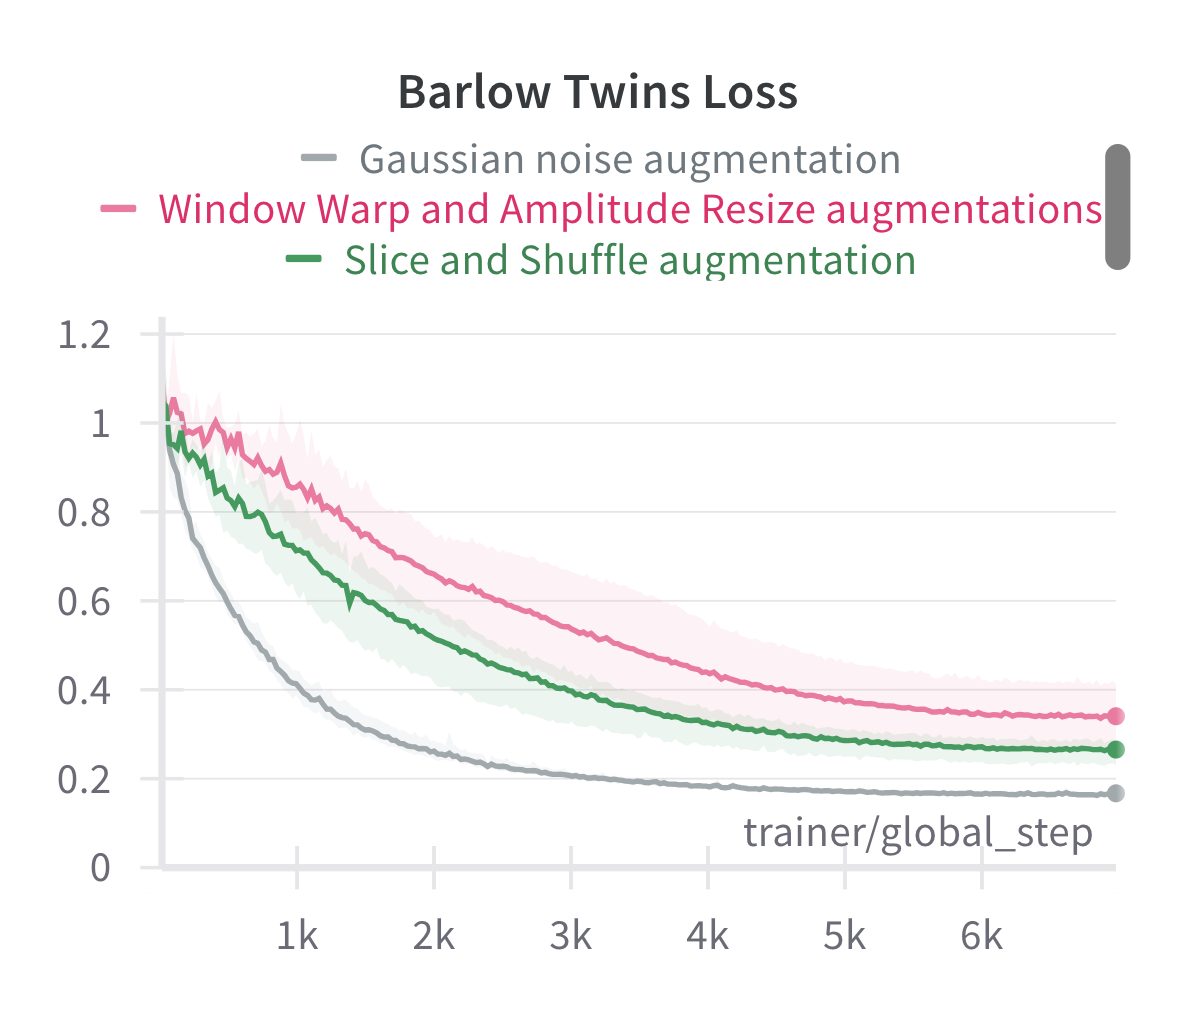
\includegraphics[width=\textwidth]{BT_loss_Uwave.png}
    \end{minipage}
    \hfill
    \begin{minipage}[b]{0.49\textwidth}
        \centering
        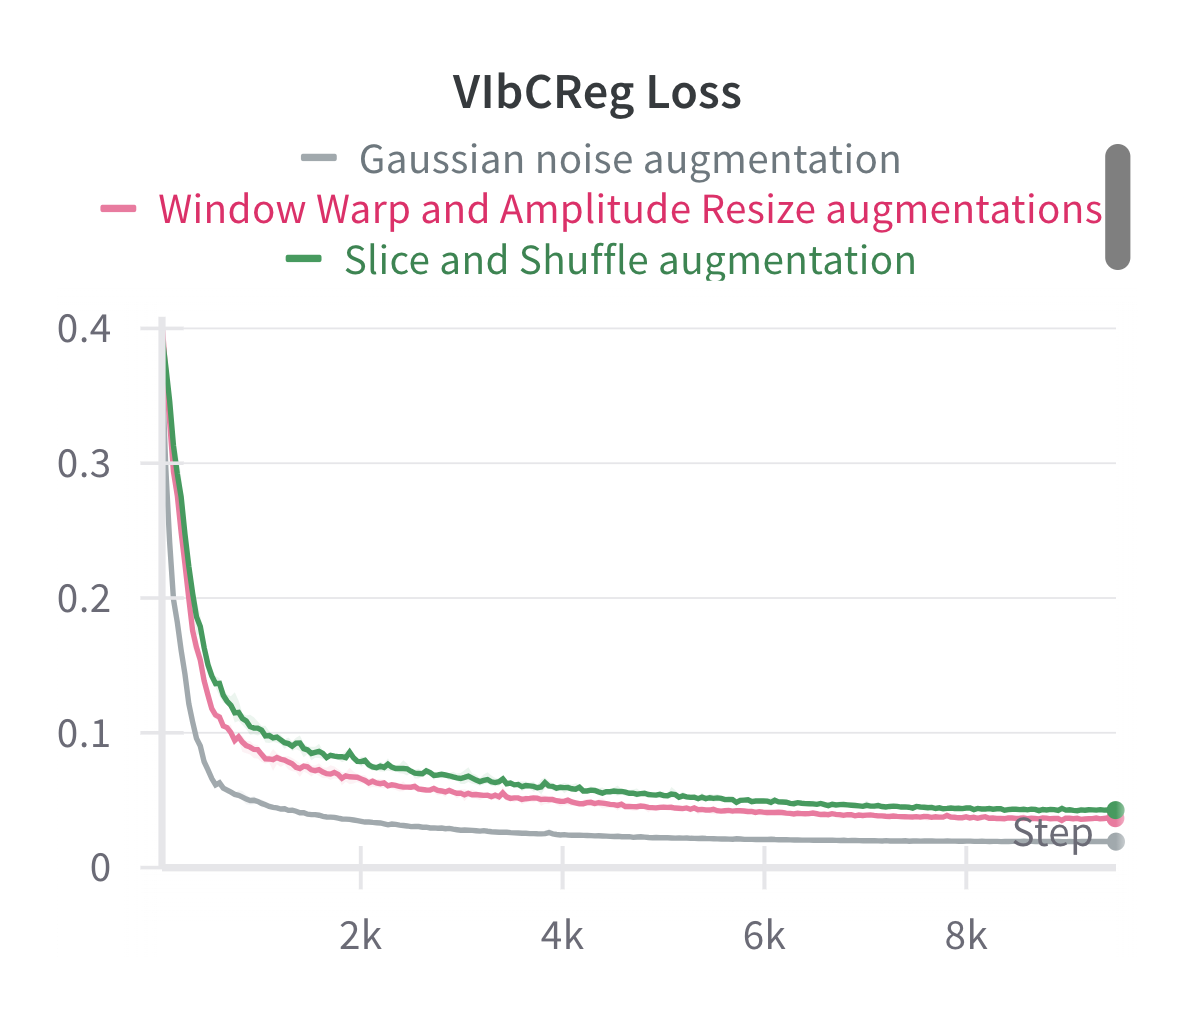
\includegraphics[width=\textwidth]{vib_loss_Uwave.png}
    \end{minipage}
    \caption{SSL loss during training on UWaveGestureLibraryAll. Averaged across four runs.}
    \label{fig:SSL_loss_UWave}
\end{figure}

We see that the Gaussian augmentation results in a SSL loss which is easier to minimize, which might be attributed to the fact that it affects the samples in a more predictable way. We too see that the VIbCReg loss decreases more rapidly than the Barlow Twins loss. Both observations are seen across datasets. \newline

Previously in figure \ref{fig:Mean_probe} we have seen that the gaussian augmentation often resulted in lower probe accuracy than the other two. In figure \ref{fig:Vibcreg_loss_knn_accuracy} we see that, on the datasets with a significant increase in probe accuracy, the augmentations that result in a more challenging SSL loss typically has higher downstream classification accuracy. We also see that for a specific augmentation, the pattern is rather flat, indicating that the particular augmentation plays the most prominent role in probe accuracy. The SSL loss for a specific augmentation varies very little compared to probe accuracy. \newline

\begin{figure}[h]
    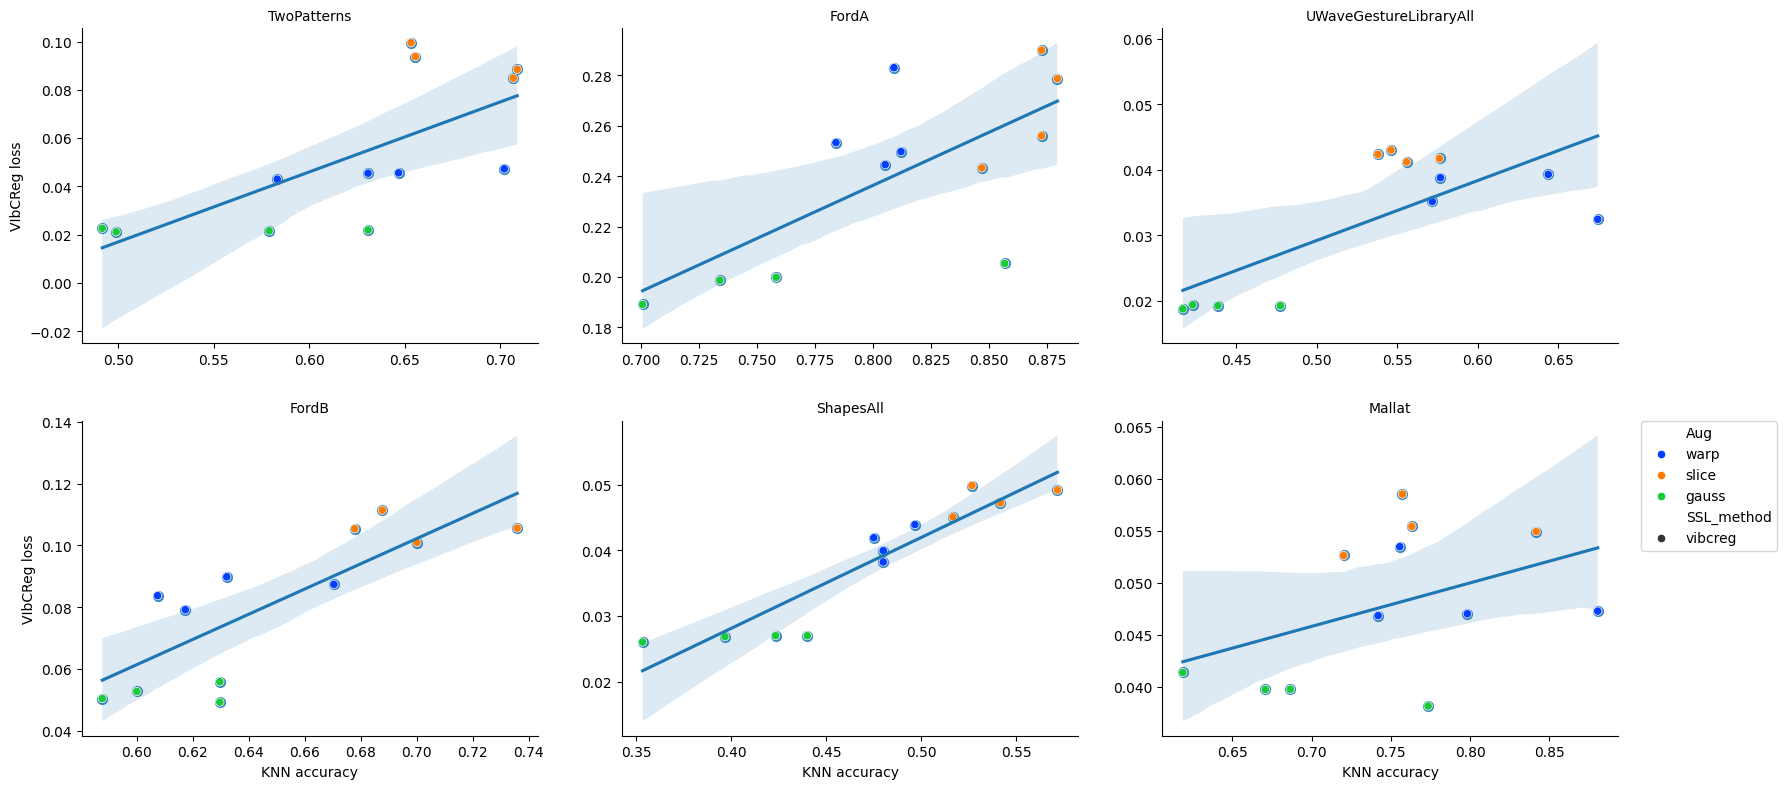
\includegraphics[scale=0.30]{Vibcreg_loss_knn_accuracy.png}
    \centering  
    \caption{KNN accuracy plotted against VIbCReg loss. Each point correspond to a single run of the model. Similar tendency is shown for Barlow Twins.}
    \label{fig:Vibcreg_loss_knn_accuracy}
\end{figure}

The training reconstruction losses are heavily minimized, both across models and augmentations. The only consistent noticeable difference is the augmented reconstruction loss, where models using Slice and Shuffle have a slightly higher loss. The differences in VQ loss for the different models is mainly due to the codebook, where we too observe that VIbCReg minimizes more effectively than Barlow Twins, and again that gaussian augmentations results in the hardest minimization followed by Window Warp and then Slice and Shuffle.\newline 

Both VIbCReg and Barlow Twins with Gaussian augmentation routinely perform on par with naive VQVAE in terms of VQ loss during training. The minimization of the codebook loss indicates that the encoder is properly aligned with the discrete latent codes. We hypothesize that when the SSL loss is not properly minimized, the encoder must adjust its weights more throughout training which keeps the encoder outputs and the discrete codes from aligning completely. 

\section{Stage 2}

For datasets with very few samples, or very few per class, the generative scores must be taken with a grain of salt. Both the classifier, and the evaluation metrics is dependent on a certain number of samples to be considered reliable. We rather look more closely on the visual inspection for these.  

\subsection{Generative quality}

The generative quality of or models are evaluated according to FID, IS and CAS. We present the top 1 and mean score across the four runs for both FID and IS in table \ref{tab:FID_IS_best} and \ref{tab:FID_IS_mean}. From the tables we see that our model produces better IS score for 12 out of 13 datates, and better FID for 10 out of 13.\newline

\begin{table}[H]
    \title{Top 1 FID and IS}
    \centering
    \begin{adjustbox}{width=\textwidth}
     \begin{tabular}{lcc|cc|cc|cc|cc|cc|cc} % 15 cols, 1 for dataset, 14 for svm/knn across models (7 models)
        \toprule
        \multirow{4}{*}{\textbf{Dataset}} & \multicolumn{2}{c}{\textbf{Baseline}} & \multicolumn{12}{c}{\textbf{SSL Method}} \\
                                            \cmidrule(lr){2-3} \cmidrule(lr){4-15}
                                          & \multicolumn{2}{c}{Regular}           & \multicolumn{6}{c}{Barlow Twins}                                                 &  \multicolumn{6}{c}{VIbCReg} \\
                                          \cmidrule(lr){2-3} \cmidrule(lr){4-9} \cmidrule(lr){10-15}
                                          &   \multicolumn{2}{c}{None}            & \multicolumn{2}{c}{Warp}  & \multicolumn{2}{c}{Slice} & \multicolumn{2}{c}{Gauss} & \multicolumn{2}{c}{Warp} & \multicolumn{2}{c}{Slice} & \multicolumn{2}{c}{Gauss} \\
                                          \cmidrule(lr){2-3} \cmidrule(lr){4-5} \cmidrule(lr){6-7} \cmidrule(lr){8-9} \cmidrule(lr){10-11} \cmidrule(lr){12-13}\cmidrule(lr){14-15}
                                          & FID$\downarrow$ & IS$\uparrow $                             & FID$\downarrow$ & IS$\uparrow$                  & FID$\downarrow$ & IS$\uparrow$                & FID$\downarrow$ & IS$\uparrow$                 & FID$\downarrow$ & IS$\uparrow$                 & FID$\downarrow$ & IS $\uparrow$                 & FID$\downarrow$ & IS$\uparrow$   \\
        \midrule
        FordA                   & 2.59 & 1.30 & 1.93 & \textbf{1.51} & 2.13 & 1.48 & 1.80 & \textbf{1.51} & 2.83 & 1.38 & 2.50 & 1.43 & \textbf{1.66} & 1.41 \\
        ElectricDevices         & 12.05 & 3.97 & 11.82 & 4.20 & \textbf{8.91} & 4.07 & 9.89 & 3.86 & 12.38 & \textbf{4.23} & 11.08 & 3.94 & 13.96 & 3.71 \\
        StarLightCurves         & \textbf{0.74} & 1.99 & 0.89 & \textbf{2.43} & 1.50 & 2.36 & 0.75 & 2.39 & 0.92 & 2.39 & 0.85 & \textbf{2.40} & 0.79 & 2.26 \\
        Wafer                   & 5.27 & \textbf{1.39} & 3.31 & 1.29 & 3.82 & \textbf{1.26} & 2.77 & 1.35 & 3.33 & 1.29 & 3.60 & 1.30 & \textbf{2.52} & 1.34 \\
        ECG5000                 & 1.56 & 2.01 & 2.43 & 2.02 & 2.27 & 2.00 & 2.15 & 2.02 & 2.15 & \textbf{2.03} & 2.21 & 2.00 & \textbf{1.52} & 2.02 \\
        TwoPatterns             & 3.63 & 2.47 & 3.59 & 2.65 & 2.74 & 2.73 & \textbf{2.24} & 2.70 & 3.45 & 2.64 & 2.90 & 2.70 & \textbf{2.19} & \textbf{2.77} \\
        UWaveGestureLibraryAll  & 8.16 & 2.24 & 6.45 & 2.94 & \textbf{6.26} & \textbf{3.13} & 7.31 & 2.79 & 6.52 & 2.99 & 6.33 & 3.06 & 7.09 & 2.79 \\
        FordB                   & 2.92 & 1.52 & 2.10 & 1.52 & 2.44 & 1.61 & 1.93 & \textbf{1.67} & 1.76 & 1.65  & 2.12 & 1.64 & \textbf{1.66} & 1.52 \\
        ShapesAll               & \textbf{21.35} & 4.32 & 35.89 & \textbf{5.22} & 29.61 & 5.16 & 27.91 & 4.83 & 30.03 & 4.95 & 31.59 & 4.92 & 27.20 & 4.94 \\
        SonyAIBORobotSurface1   & 18.21 & 1.27 & 26.20 & 1.32 & 28.90 & 1.28 & 21.63 & 1.32 & 21.98 & 1.36 & 25.20 & 1.38 & \textbf{15.73} & \textbf{1.55} \\
        SonyAIBORobotSurface2   & 3.85 & 1.69 & 2.50 & 1.82 & 3.34 & 1.79 & \textbf{0.82} & 1.82 & 2.61 & 1.81 & 2.75 & 1.83 & 1.24 & \textbf{1.84} \\
        Symbols                  & 8.50 & 2.43 & 5.86 & 3.20 & 7.39 & 2.82 & \textbf{4.25} & \textbf{3.50} & 6.78 & 3.39 & 7.21 & 3.23 & 8.21 & 3.30 \\
        Mallat                   & \textbf{1.31} & 3.41 & 2.01 & 3.67 & 2.24 & 3.72 & 1.85 & 3.66 & 1.87 & 3.34 & 2.30 & 3.05 & \textbf{1.31} & \textbf{3.92} \\
        \bottomrule
    \end{tabular}
    \end{adjustbox}
    \caption{Summary of FID and IS scores by SSL Method and Augmentation. Best achieved results are highlighted in bold}
    \label{tab:FID_IS_best}
\end{table}


\begin{table}[h]
    \centering
    \title{Mean FID and IS}
    \begin{adjustbox}{width=\textwidth}
     \begin{tabular}{lcc|cc|cc|cc|cc|cc|cc} % 15 cols, 1 for dataset, 14 for svm/knn across models (7 models)
        \toprule
        \multirow{4}{*}{\textbf{Dataset}} & \multicolumn{2}{c}{\textbf{Baseline}} & \multicolumn{12}{c}{\textbf{SSL Method}} \\
                                            \cmidrule(lr){2-3} \cmidrule(lr){4-15}
                                          & \multicolumn{2}{c}{Regular}           & \multicolumn{6}{c}{Barlow Twins}                                                 &  \multicolumn{6}{c}{VIbCReg} \\
                                          \cmidrule(lr){2-3} \cmidrule(lr){4-9} \cmidrule(lr){10-15}
                                          &   \multicolumn{2}{c}{None}            & \multicolumn{2}{c}{Warp}  & \multicolumn{2}{c}{Slice} & \multicolumn{2}{c}{Gauss} & \multicolumn{2}{c}{Warp} & \multicolumn{2}{c}{Slice} & \multicolumn{2}{c}{Gauss} \\
                                          \cmidrule(lr){2-3} \cmidrule(lr){4-5} \cmidrule(lr){6-7} \cmidrule(lr){8-9} \cmidrule(lr){10-11} \cmidrule(lr){12-13}\cmidrule(lr){14-15}
                                          & FID$\downarrow$ & IS$\uparrow $                             & FID$\downarrow$ & IS$\uparrow$                  & FID$\downarrow$ & IS$\uparrow$                & FID$\downarrow$ & IS$\uparrow$                 & FID$\downarrow$ & IS$\uparrow$                 & FID$\downarrow$ & IS $\uparrow$                 & FID$\downarrow$ & IS$\uparrow$   \\
        \midrule
        FordA                   & 5.15 & 1.16 & 2.59 & 1.41 & 2.36 &\textbf{ 1.45} & \textbf{2.28} & \textbf{1.45} & 3.01 & 1.34 & 2.90 & 1.41 & 3.73 & 1.29 \\
        ElectricDevices         & 13.48 & 3.75 & 16.51 & 3.95 & \textbf{10.20} & 3.93 & 11.54 & 3.75 & 13.99 & \textbf{4.17} & 11.82 & 3.85 & 15.20 & 3.55 \\
        StarLightCurves         & \textbf{1.01} & 1.93 & 1.29 & 2.35 & 1.91 & 2.32 & 1.08 & 2.25 & 1.07 & 2.35 & 1.19 & \textbf{2.36} & 1.05 & 2.22 \\
        Wafer                   & 5.72 & \textbf{1.33} & 3.70 & 1.25 & 4.20 & 1.24 & 2.85 & 1.31 & 3.67 & 1.26 & 3.86 & 1.26 & \textbf{2.84} & 1.31 \\
        ECG5000                 & \textbf{1.62} & 1.94 & 2.61 & \textbf{2.00} & 2.56 & 1.98 & 2.47 & \textbf{2.00} & 2.60 & 1.99 & 2.39 & \textbf{2.00} & 1.76 & 1.99 \\
        TwoPatterns             & 4.04 & 2.41 & 4.00 & 2.54 & 2.96 & 2.66 & \textbf{2.44} & \textbf{2.67} & 4.05 & 2.56 & 3.15 & 2.66 & 2.62 & \textbf{2.67} \\
        UWaveGestureLibraryAll  & 8.48 & 2.13 & 6.77 & 2.86 & 6.64 & 2.96 & 7.35 & 2.73 & 6.80 & 2.91 & \textbf{6.49} & \textbf{2.99} & 7.34 & 2.72 \\
        FordB                   & 4.05 & 1.28 & 2.66 & 1.48 & 3.49 & 1.50 & 2.88 & \textbf{1.52} & \textbf{2.49} & 1.48 & 3.07 & 1.51 & 3.04 & 1.31 \\
        ShapesAll               & \textbf{27.64} & 4.22 & 38.22 & 5.07 & 32.54 & \textbf{5.04} & 32.25 & 4.56 & 36.59 & 4.72 & 35.79 & 4.76 & 31.56 & 4.71 \\
        SonyAIBORobotSurface1   & 23.71 & 1.20 & 30.65 & 1.22 & 31.97 & 1.21 & 25.29 & 1.28 & 26.11 & 1.32 & 28.20 & 1.32 & \textbf{18.61} & \textbf{1.44} \\
        SonyAIBORobotSurface2   & 5.42 & 1.62 & 3.35 & 1.77 & 4.41 & 1.74 & \textbf{1.78} & \textbf{1.81} & 4.43 & 1.74 & 3.32 & 1.79 & 2.36 & 1.79 \\
        Symbols                 & 13.62 & 1.99 & 9.78 & 2.92 & 9.78 & 2.67 & 8.61 & 3.14 & 8.84 & 3.20 & 9.74 & 3.03 & \textbf{8.58} & \textbf{3.24} \\
        Mallat                  & 2.09 & 3.01 & 2.54 & 3.29 & 3.68 & 2.94 & 2.12 & 3.53 & 2.11 & 3.18 & 2.40 & 2.96 & \textbf{1.65} & \textbf{3.72} \\
        \bottomrule
    \end{tabular}
    \end{adjustbox}
    \caption{Summary of FID and IS scores by SSL Method and Augmentation. Best mean achieved FID and IS are highlighted in bold}
    \label{tab:FID_IS_mean}
\end{table}

In figure \ref{fig:mean_gen_scores} we get a better overview of the results, and observe that both Barlow Twins and VIbCReg produces better samples than the naive VQVAE in terms of FID and IS.
Additionally we see that the use of gaussian augmentation results in the largest improvements for most datasets. The high IS scores indicate that NC-VQVAE captures the conditional distributions better than naive VQVAE in many datasets. This will be explored further in section \ref{section:Visual inspection}. The improved FID scores indicates that the synthetic samples more closely resemble the test data. The moderate decrease in FID, compared to the increase in IS, could indicate that the generated samples does not generalize too well to the test data. The discrete latent representations from NC-VQVAE provides more information regarding the classes, as we saw from the improved downstream classification accuracy in stage 1. This additional class specific information seems to assist the prior learning in capturing class conditional distributions.

\begin{figure}[H]
    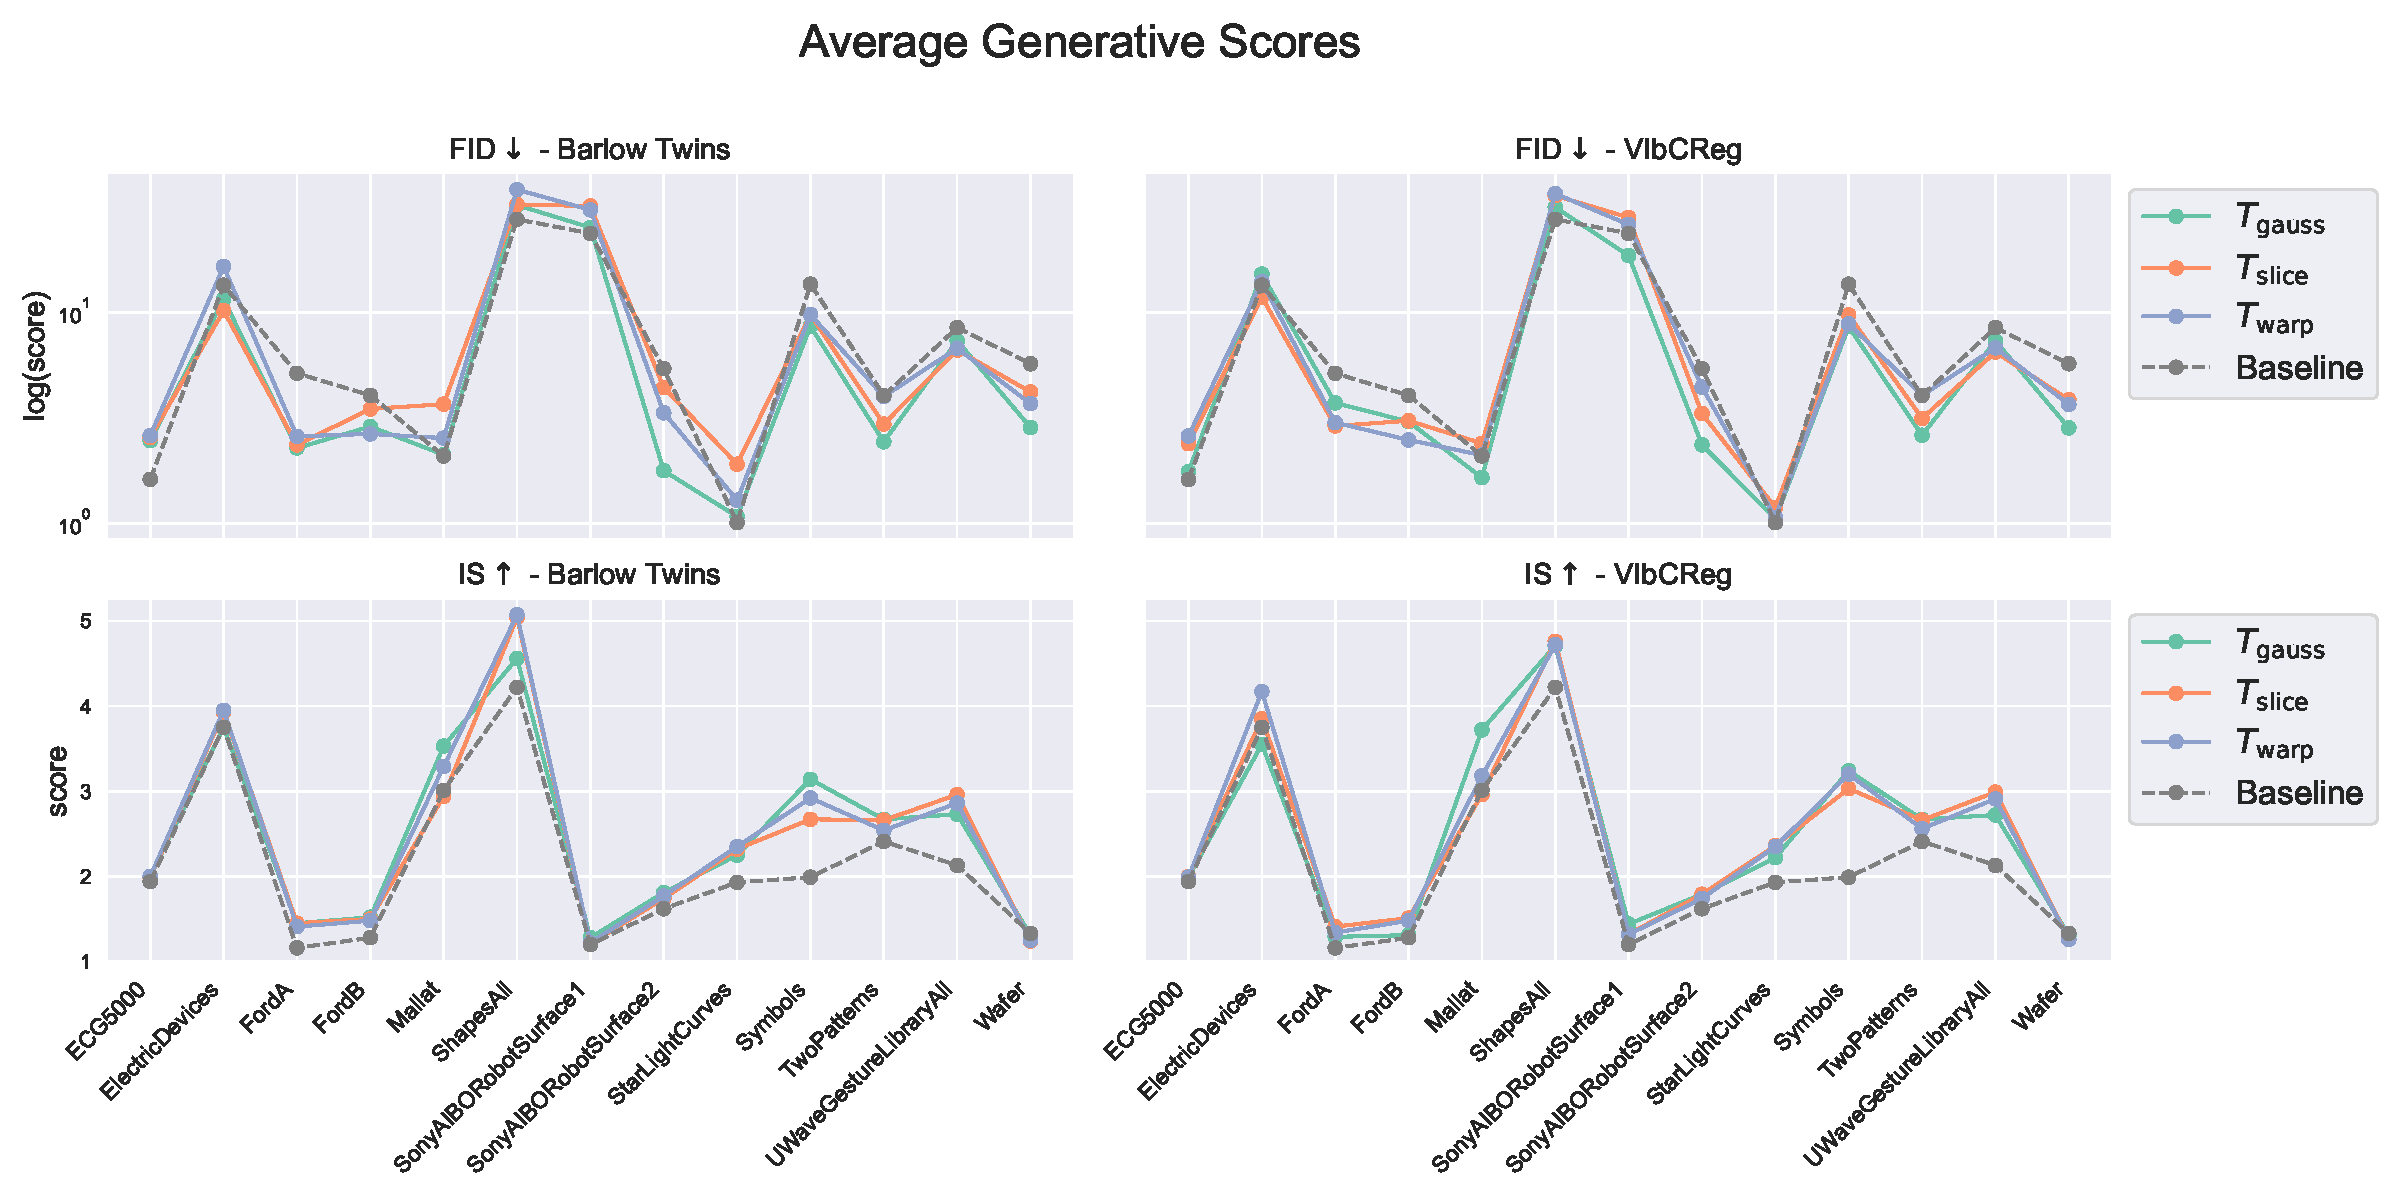
\includegraphics[scale=0.35]{gen_scores.pdf}
    \centering  
    \caption{Mean FID and IS scores for Barlow Twins and VIbCReg VQVAE. FID is plotted on a log scale because of the large difference in values across datasets.}
    \label{fig:mean_gen_scores}
\end{figure}

It is worth mentioning that the FID and IS score is calculated using the SupervisedFCN, which is also trained on the UCR Archive. Thus, the FID and IS scores could have a bias toward samples that mimic the training data. 


\subsection{Class conditional sampling}
\TODO{How do we calculate the CAS? How many samples etc.}

We present the mean CAS for all models across datasets in table \ref{tab:mean_cas}.

\begin{table}[H]
    \centering
    \title{Mean CAS}
    \begin{adjustbox}{width=\textwidth}
    \begin{tabular}{lc|c|c|c|c|c|c} % 8 cols, 1 for dataset, 7 for val_recons across models (7 models)
        \toprule
        \multirow{3}{*}{\textbf{Dataset}} & \multicolumn{1}{c}{\textbf{Baseline}} & \multicolumn{6}{c}{\textbf{SSL Method}} \\
                                         \cmidrule(lr){3-8}
                                          & \multicolumn{1}{c}{Regular}           & \multicolumn{3}{c}{Barlow Twins}    &  \multicolumn{3}{c}{VIbCReg} \\
                                                                                   \cmidrule(lr){3-5}                    \cmidrule(lr){6-8}
                                          &   None                                & Warp  & Slice & Gauss               & Warp & Slice & Gauss \\
                            
        \midrule
        FordA                   & 0.864 & 0.884 & \textbf{0.902} & 0.878 & 0.864 & 0.895 & 0.870 \\
        ElectricDevices         & 0.614 & 0.588 & 0.607 & 0.599 & \textbf{0.618} & 0.610 & 0.594 \\
        StarLightCurves         & 0.960 & 0.953 & 0.955 & \textbf{0.965} & 0.962 & 0.954 & 0.964 \\
        Wafer                   & 0.976 & 0.977 & 0.978 & 0.968 & 0.979 & 0.976 & \textbf{0.984} \\
        ECG5000                 & 0.866 & 0.881 & 0.863 & 0.880 & 0.877 & 0.892 & \textbf{0.910} \\
        TwoPatterns             & 0.808 & 0.770 & 0.788 & \textbf{0.847} & 0.715 & 0.781 & 0.846 \\
        UWaveGestureLibraryAll  & 0.333 & 0.300 & 0.367 & 0.313 & 0.360 & \textbf{0.401} & 0.383 \\
        FordB                   & 0.725 & 0.748 & \textbf{0.756} & 0.741 & 0.750 & 0.738 & 0.750 \\
        ShapesAll               & 0.361 & 0.344 & 0.329 & \textbf{0.420 }& 0.379 & 0.367 & 0.404 \\
        SonyAIBORobotSurface1   & 0.975 & 0.933 & 0.957 & 0.979 & 0.982 & 0.976 & \textbf{0.985} \\
        SonyAIBORobotSurface2   & 0.929 & 0.956 & 0.951 & 0.969 & 0.960 & \textbf{0.970} & 0.964 \\
        Symbols                 & 0.956 & 0.929 & 0.930 & 0.930 & 0.969 & \textbf{0.974} & 0.963 \\
        Mallat                  & 0.471 & 0.642 & 0.563 & 0.661 & 0.827 & 0.876 & \textbf{0.908} \\
        \bottomrule
    \end{tabular}
    \end{adjustbox}
    \caption{Mean CAS score across datasets. Results averaged across four runs.}
    \label{tab:mean_cas}
\end{table}

We see that some configuration of NC-VQVAE outperforms the naive VQVAE on all datasets, as well as VIbCReg with gaussian augmentation outperforming the baseline on 12 out of 13, where the one dataset where it falls short its within one percent. In general we observe that NC-VQVAE performs well across all datasets, and in particular with gaussian augmentation. The dataset where we see the most dramatic increase is Mallat, with an improvement of $0.437$. This particular case will be investigated in section \ref{section:Visual inspection}.  

\begin{figure}[h]
    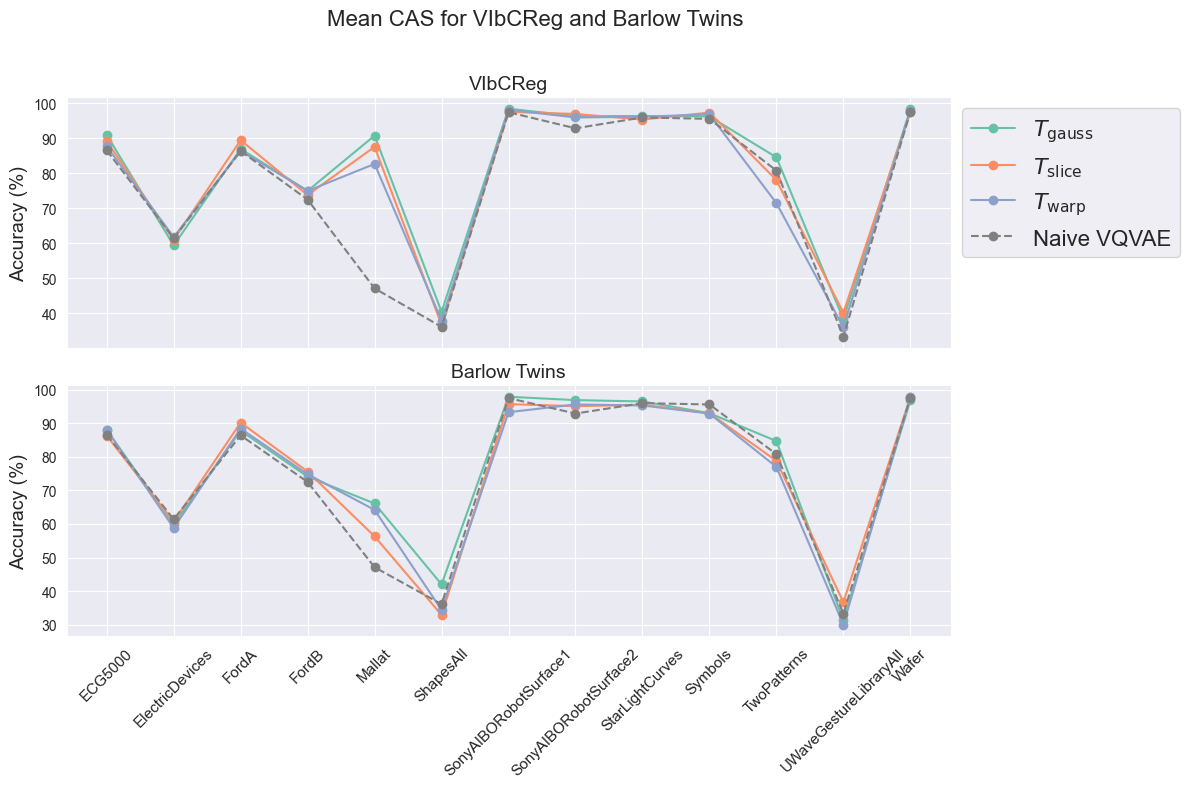
\includegraphics[scale=0.4]{Mean_CAS.png}
    \centering  
    \caption{Mean CAS across all datasets.}
    \label{fig:Mean_CAS}
\end{figure}





\subsection{Prior loss}
Mention that during experiments with our stage 2 modification, embed / finetune, we observed that the val prior loss with our modification was higher, but with similar shape as without. If we had time and computational resources to rerun the experiments, then we would omit the stage 2 modification. The FID/IS in our main experiments are in many cases better than baseline VQVAE, despite higher val prior loss.
\newline

Naive VQVAE outperforms NC-VQVAE in terms of validation prior loss across datasets. There is the occasional dataset where a model with gaussian augmentation performs equally well. The minimization of the validation prior loss does therefore not correspond to improved synthetic samples in general.



\subsection{The influence of stage 1 on stage 2}
The best performing datasets in terms of probe accuracies: "FordA", "FordB", "Mallat", "ShapesAll", "TwoPatterns", "UWaveGestureLibraryAll"\newline

Relationship between reconstruction in stage 1 and FID/IS/CAS:
Does better reconstruction capabilities in stage 1 improve the generative model?\newline

Relationship between probes in stage 1 and FID/IS/CAS:
Does better probe accuracies (class separation) in stage 1 improve the generative model?\newline

How does the best performing models from stage 1 transfer to stage 2?\newline

Look at FordA, FordB, Mallat, ShapesALL, TwoPatterns and UWaveGestureLibraryAll. The datasets where probe accuracies are good compared to baseline. Slice is aug with best performance overall on these datasets. \newline

\begin{figure}[h]
    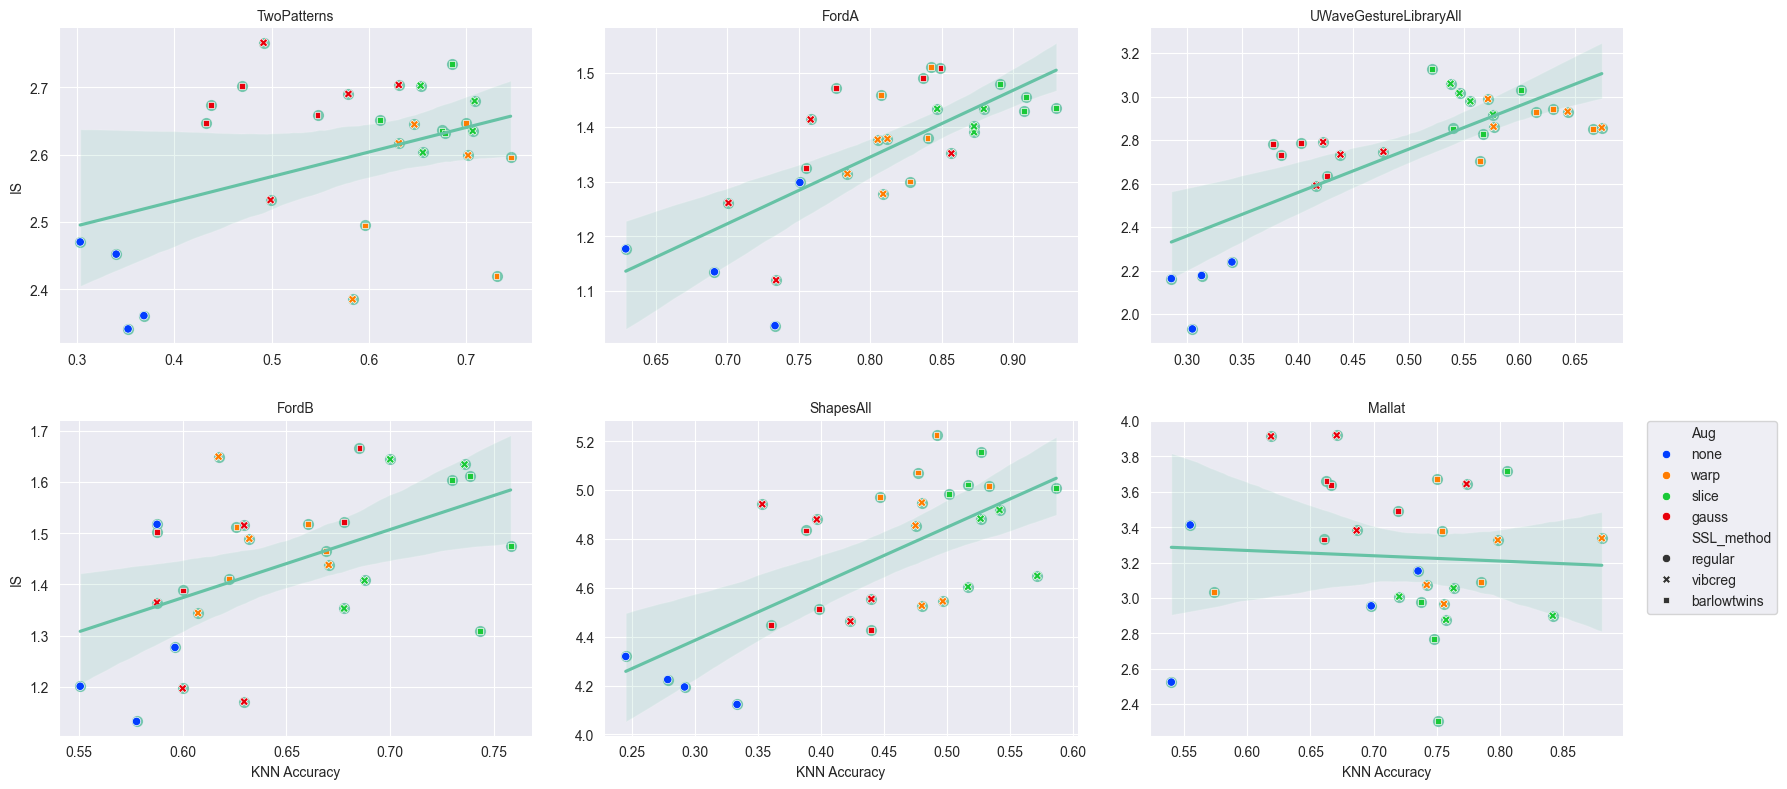
\includegraphics[scale=0.3]{KNN_IS_Subset.png}
    \centering  
    \caption{KNN plotted against Inception Score on the subset of datasets with significant improvement in probe accuracy.}
    \label{fig:KNN_IS_Subset}
\end{figure}

\begin{figure}[H]
    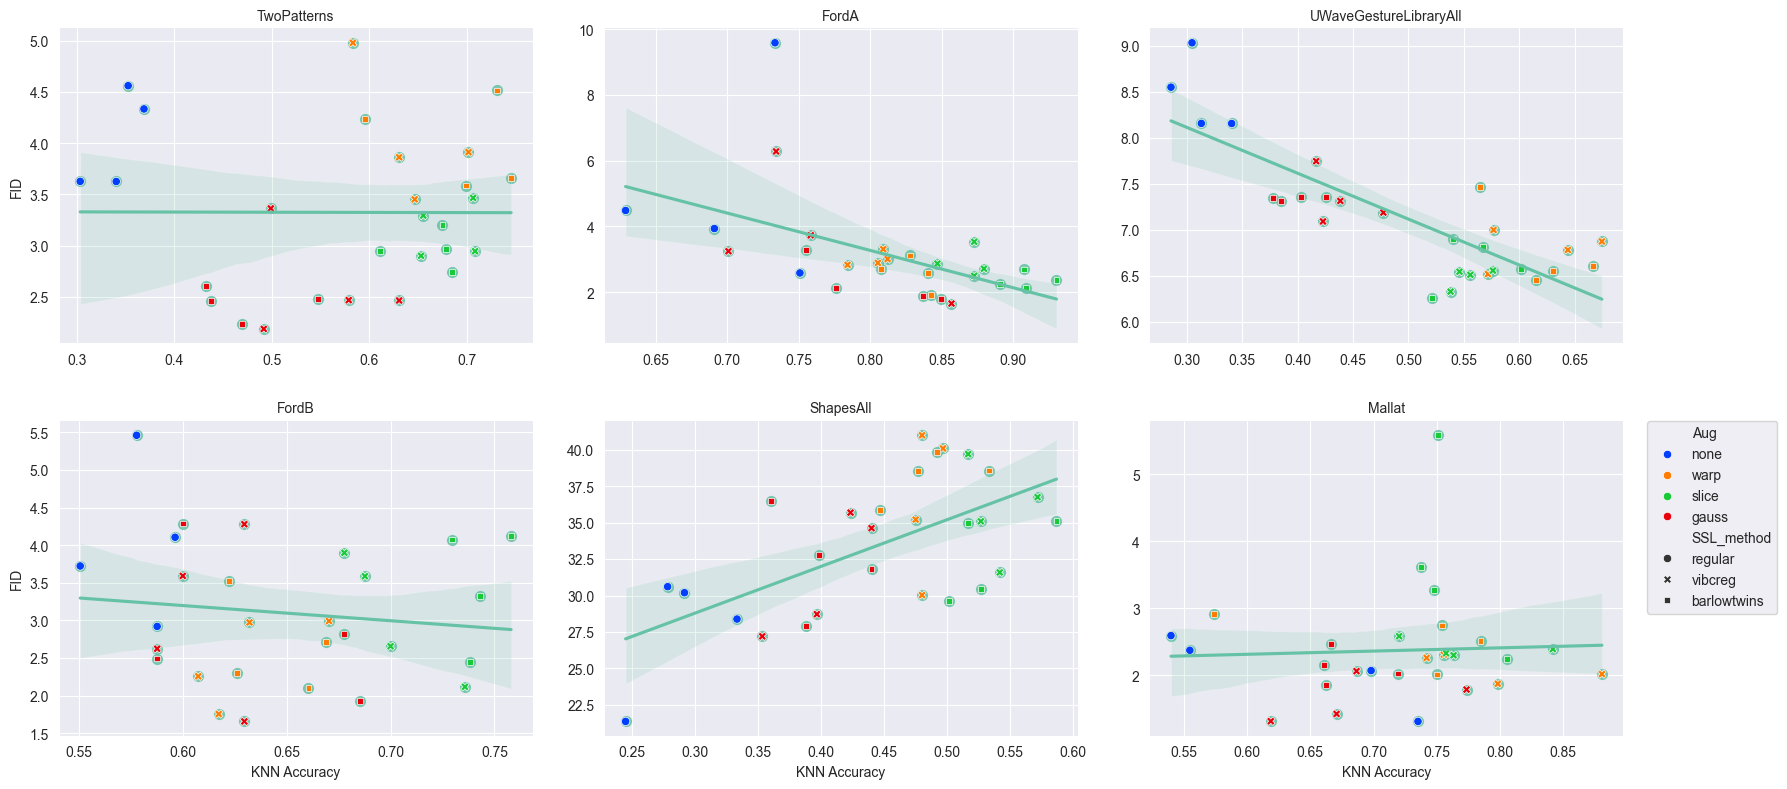
\includegraphics[scale=0.3]{KNN_FID_Subset.png}
    \centering  
    \caption{KNN plotted against Fréchet Inception Distance on the subset of datasets with significant improvement in probe accuracy.}
    \label{fig:KNN_FID_Subset}
\end{figure}

In Figure \ref{fig:KNN_IS_Subset} and \ref{fig:KNN_FID_Subset}, we see the relationship between KNN accuracy and FID/IS on the subsets where the probe accuracy is substantially improved with NC-VQVAE. The corresponding plots with SVM accuracy show similar trends. From Figure \ref{fig:KNN_IS_Subset} we see a trend, with higher probe accuracy correlating with higher IS. Upon closer inspection, we see a clear pattern of the prominent effect of augmentations. 
For each specific augmentation, the correlation between KNN and IS is close to $0$.

Particularly interesting is UWaveGestureLibraryAll.




\subsection{Token usage}
We say memorization/overfitting when the selected probabilities are mainly >0.9. 


wafer: Barlow and VIbCReg are more certain of tokens than naive. Often at time T=3 the main proportion of selected samples have probability >0.9. Barlow to a greater degree than VIbCReg.

ShapesAll: Barlow a bit more uncertain than VIbCReg. For a seed they both collapse and basically sample tokens with probability 1 from T=1.

Sony2: Barlow is much more certain earlier for several models. Both are significantly more certain than naive.

Mallat: All models overfit quite hard. VIbCReg and Barlow has some more variability, vibcreg best of SSL.

FordB: more healthy distributions. VIbCReg a bit more certain, in a good way i think.

ECG5000: For several models barlow and vib overfits hard. Naive has healty distributions, mostly. 

TwoPatterns: Naive consistently uncertain. VIbCReg and Barlow develops similarly as T increases, and looks very good. This is a prime example of what i consider good.

UWave: VIbCReg and Barlow has several cases of severe overfitting, . Naive looks healthy.

Symbols: VIbCReg has significantly more diversity than barlow. Still overfits quite a bit. Naive overfits in some cases, but generally healthier.

ElectricDevices: Similar behavior. After T=4 almost certain.

StarLightCurves: Overfitting in some cases. Otherwise a more healty distribution than naive.

Sony1: Barlow overfits more than VIbCReg . Both have some quite extreme cases. Warp produces the best distributions. 

FordA: One model each with some overfitting (both gaussian). 

Note: Does overfitting etc, happen mostly for Gauss? It is the case for StarLightCurves.

Include something on the differences in sampling/token usage between naive VQVAE and NC-VQVAE. NC-VQVAE has a tendency to be more certain of tokens selected. For small datasets such as Mallat, the certainty is close to $1$ for most sampled tokens. 

\TODO{Investigate this further. Compare/relate the selected probability histograms with token usage histograms / perplexity}

Would be interesting to investigate different values for T in maskgit iterative sampling.


Higher masking ratios during training etc.

\subsection{Visual inspection}
\label{section:Visual inspection}
In the following we present generated samples from naive VQVAE and NC-VQVAE for some selected dataset. The ground truth, both test and train, are additionally included in order to better make sense of the IS and FID scores. \newline

Some datasets, such as FordA and B, is poorly suited for this type of visual inspection, as illustrated previously in Figure \ref{fig:datasets}. As a result, the selection of datasets is primarily based on how well they lend themselves to this type of presentation.\newline

For each figure in the following sections, 50 samples are generated from each model. For the ground truth, we plot a subset of 50 randomly selected samples, or the entire set if the dataset contain less than 50 samples.\newline

Typically naive VQVAE has more trouble with capturing the global consistency of the samples when samples are scarce and diverse, as seen on ShapesAll and Symbols. In contrast, our method will tend to overfit in these cases. The overfitting issue is most prominent in the class conditional distributions. \newline

There are only minor differences seen in the generated samples form NC-VQVAE trained with different augmentations, especially when sample size is low.\newline

\subsubsection{ECG5000}

In Figure \ref{fig:Warp_ECG5000} we present generated samples from naive VQVAE and NC-VQVAE trained with Window Warp and Amplitude Resize augmentations on ECG5000.\newline

We see some evidence that VIbCReg maintains more variability than Barlow Twins, particularly in class 1 and 2. \newline

In class 4, where the training data only consists of 2 samples, both Barlow Twins and VIbCReg catches the pattern, while producing some variation which resemble the training samples. The naive VQVAE samples does not capture this distribution, but when compared to the test data, it is more similar, which again could explain why naive VQVAE performs slightly better in terms of FID score than NC-VQVAE. \newline

The ability of NC-VQVAE to accurately model the conditional distributions and their characteristics, is evidence for why CAS was slightly higher than for naive VQVAE.


\begin{figure}[H]
    \centering
    % \hfill
    \begin{minipage}[b]{0.32\textwidth}
        \centering
        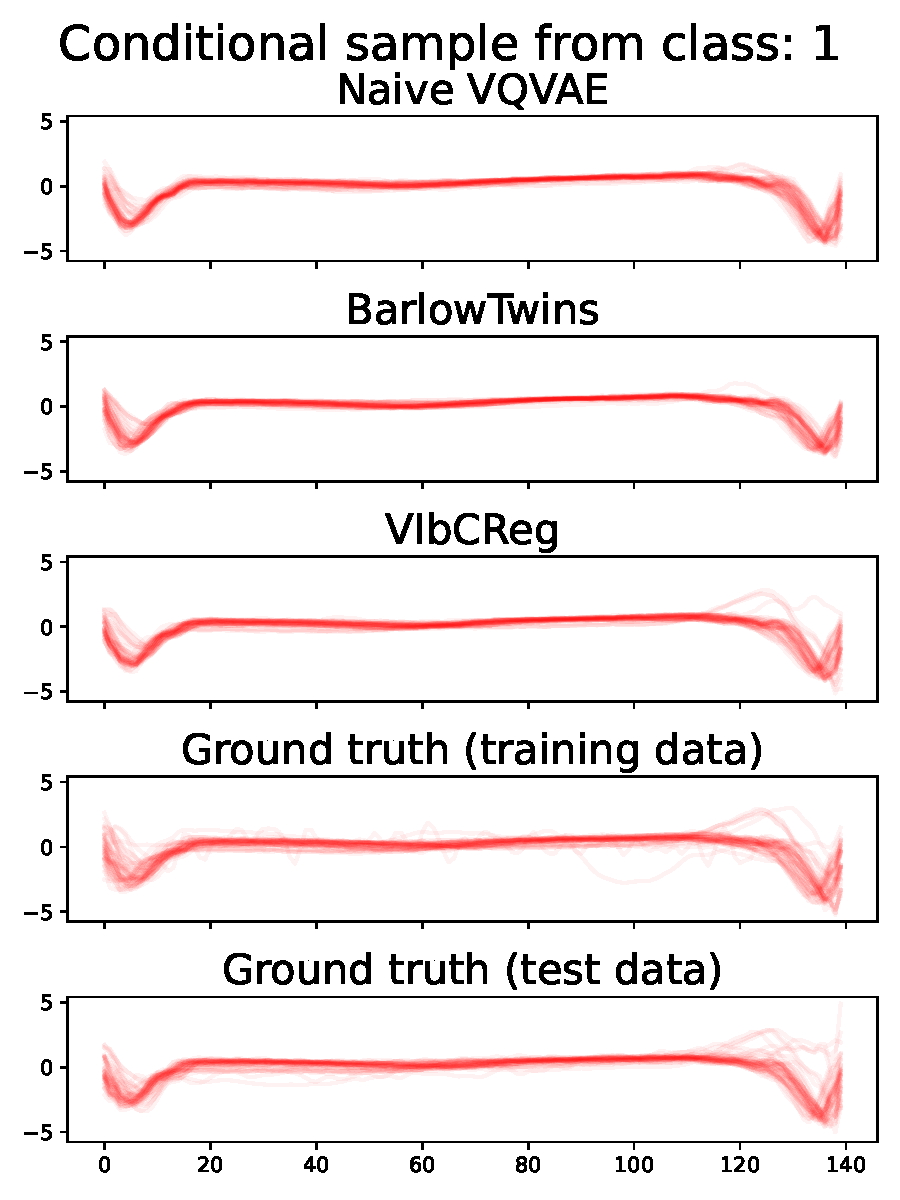
\includegraphics[width=\textwidth]{ECG5000-conditional-class1.pdf}
    \end{minipage}
    \begin{minipage}[b]{0.32\textwidth}
        \centering
        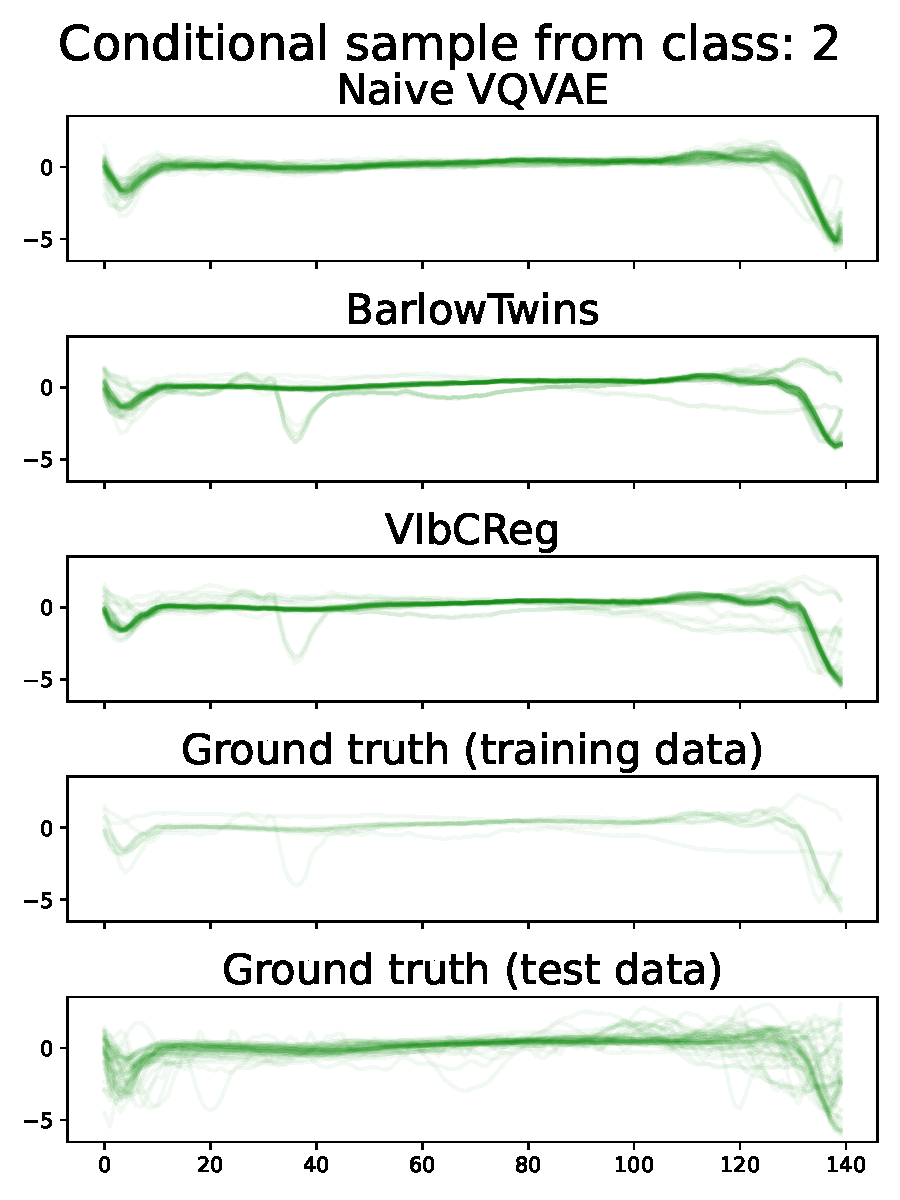
\includegraphics[width=\textwidth]{ECG5000-conditional-class2.pdf}
    \end{minipage}
    \begin{minipage}[b]{0.32\textwidth}
        \centering
        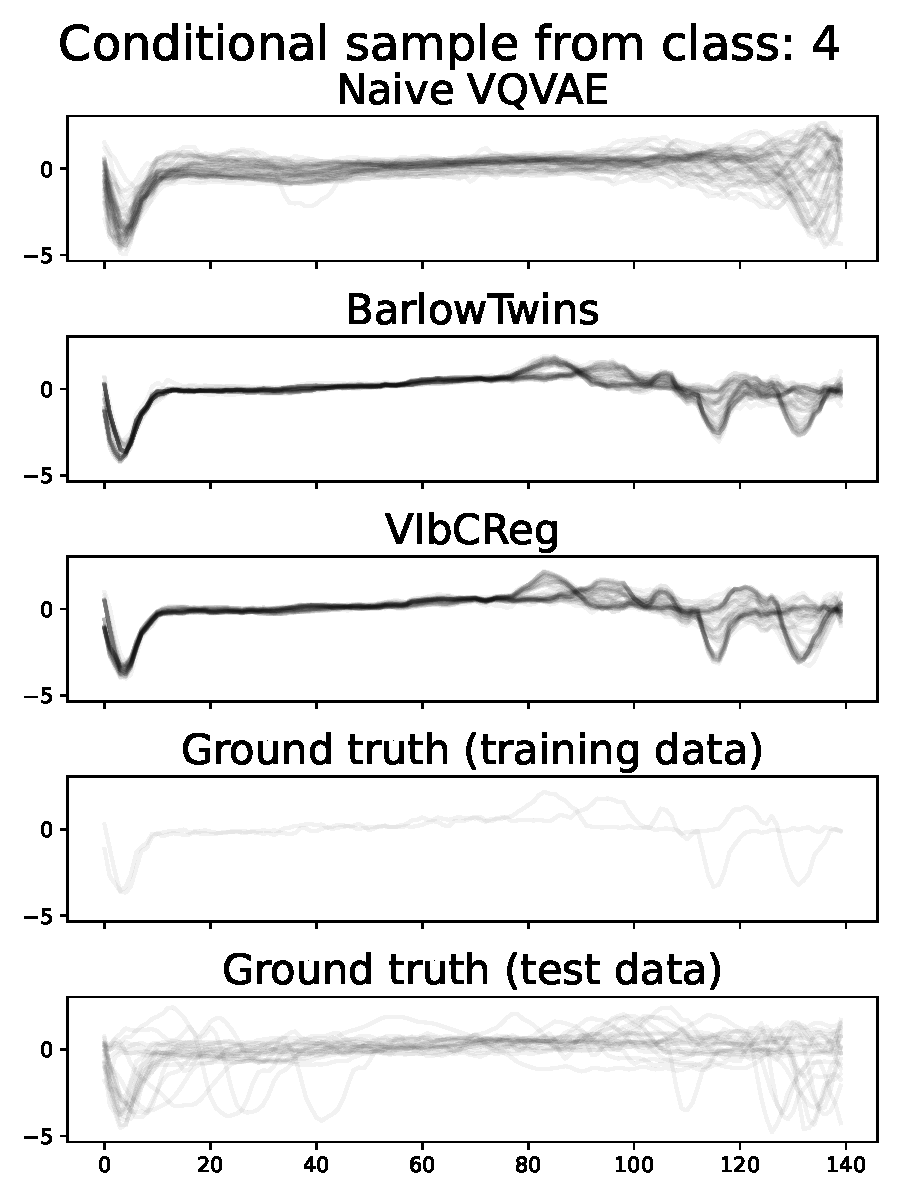
\includegraphics[width=\textwidth]{ECG5000-conditional-class4.pdf}
    \end{minipage}
    \caption{Class conditional distribution for some selected classes of ECG5000. Barlow and VIbCReg both trained with window warp and amplitude resize augmentations. 50 samples from each model.}
    \label{fig:Warp_ECG5000}
\end{figure}


\subsubsection{Mallat}
Mallat is a simulated dataset, where the classes have very little variability and training and test distribution are indistinguishable, except for sample size. \newline

We observe that VIbCReg is superior in capturing the variability, compared to Barlow Twins and naive VQVAE. This is most evident in the first 300 timesteps of class 5 in Figure \ref{fig:Gaussian_Mallat}. Looking as class 7, we see Barlow Twins completely collapsing, essentially producing the same sample over and over. \newline

These illustrations explains the significant increase in CAS seen in Figure \ref{fig:Mean_CAS}, particularly for VIbCReg. It too explains how VIbCReg both increases IS and reduces FID. \newline



\TODO{TSNE/PCA}

\begin{figure}[H]
    \centering
    \begin{minipage}[b]{0.32\textwidth}
        \centering
        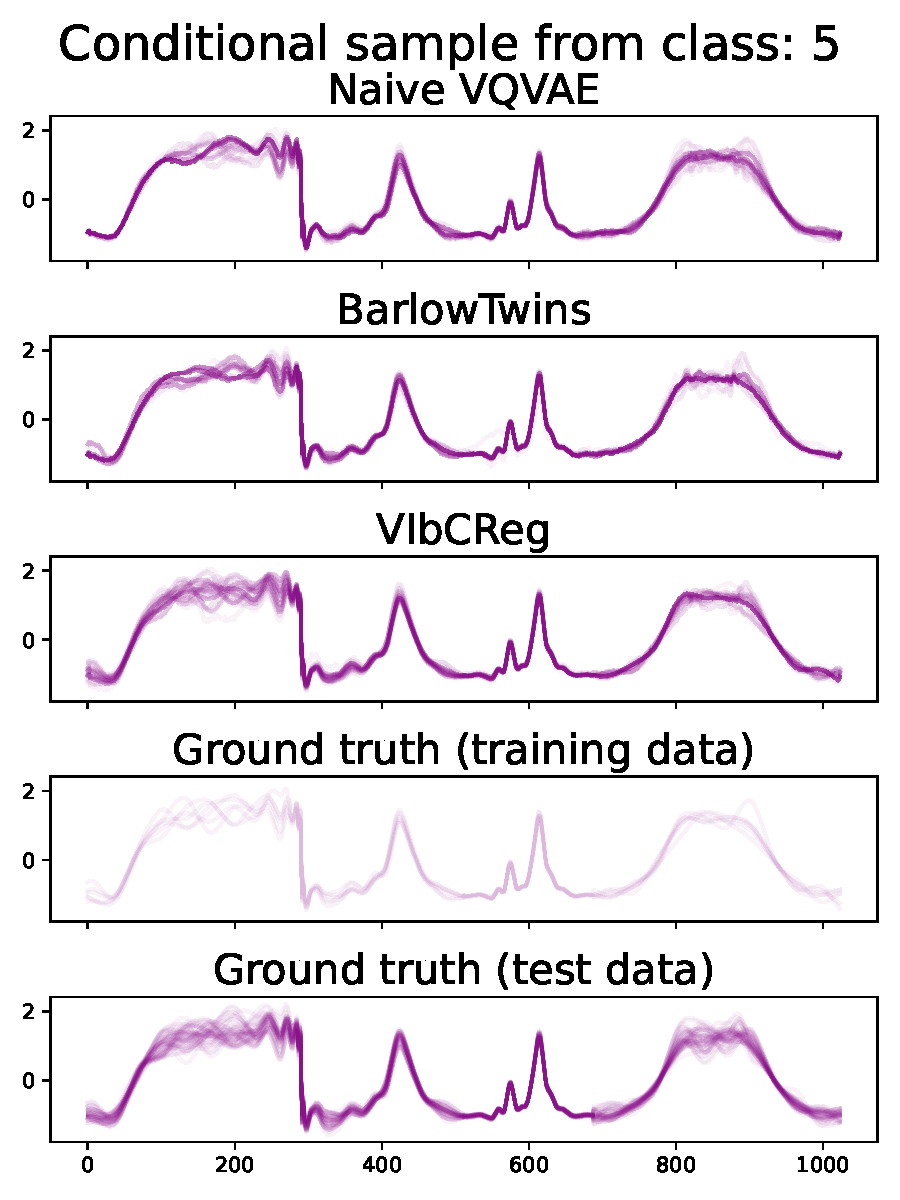
\includegraphics[width=\textwidth]{Mallat-conditional-class5.pdf}
    \end{minipage}
    % \hfill
    \begin{minipage}[b]{0.32\textwidth}
        \centering
        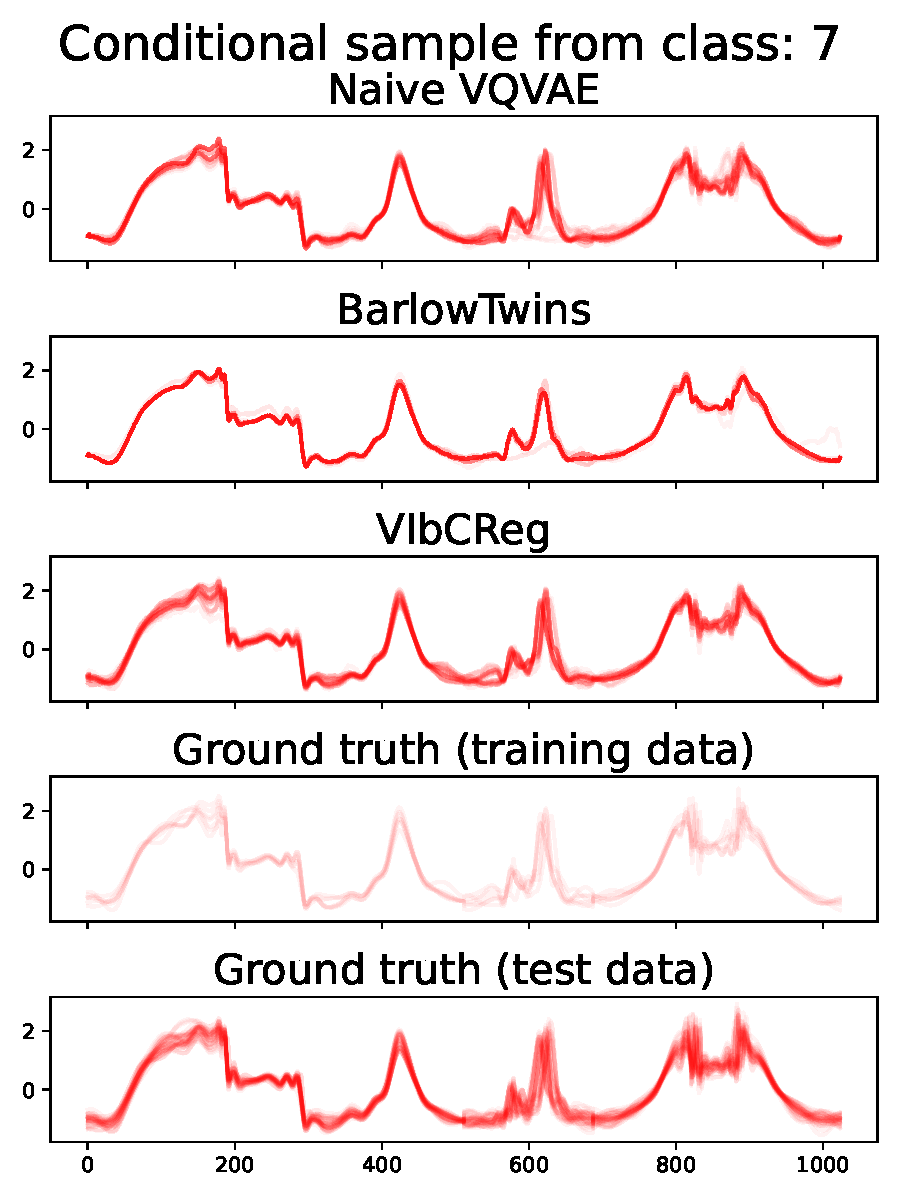
\includegraphics[width=\textwidth]{Mallat-conditional-class7.pdf}
    \end{minipage}
    \begin{minipage}[b]{0.32\textwidth}
        \centering
        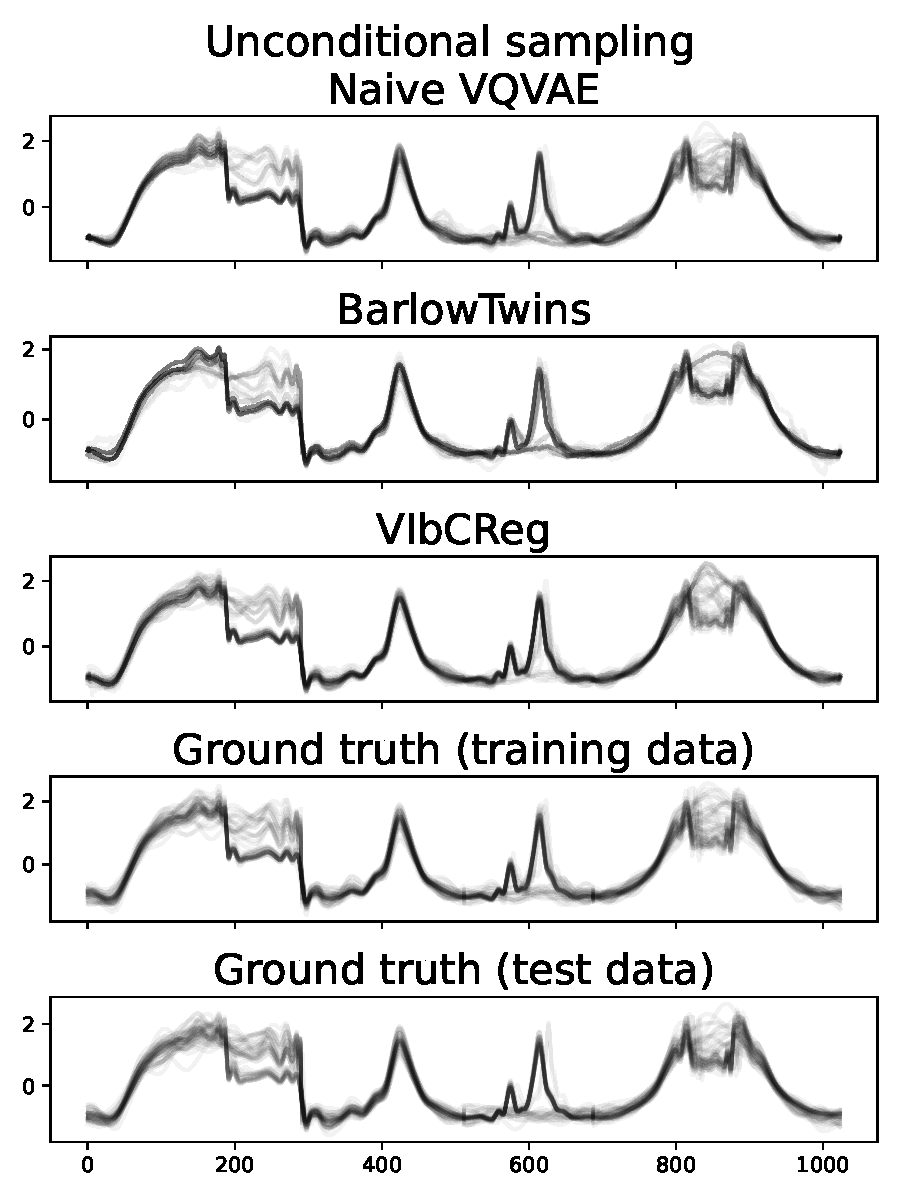
\includegraphics[width=\textwidth]{Mallat-unconditional.pdf}
    \end{minipage}
    \caption{Class conditional distribution for some selected classes of Mallat, in addition to unconditional samples. Barlow and VIbCReg both trained with gaussian augmentation.}
    \label{fig:Gaussian_Mallat}
\end{figure}


\subsubsection{Symbols}

The Symbols dataset consists of several distinct, but simple, patterns. For each class there is less than 5 training samples.

In Figure \ref{fig:Gauss_Symbols}, particularly the unconditional sample, we see that naive VQVAE does not capture the entire underlying distribution, some classes are not represented/not recognizable, while global consistency for the sinusoids are poor, particularly towards the end.\newline

In class 3, we observe that both Barlow Twins and VIbCReg mimic the training data to a large degree,VIbCReg to a slightly higher degree than Barlow Twins. At first glance the naive VQVAE looks to produce the most desirable distribution, but upon closer inspection we see an excessive amount of noise and lack of consistency.\newline

The IS on Symbols, for both VIbCReg and BarlowTwins, is substantially higher than naive VQVAE. While this is not surprising after inspecting the samples, it exposes an issue with the IS metric. It fails to take intraclass diversity into account, and is therefore oblivious to overfitting. \newline

\begin{figure}[H]
    \centering
    \begin{minipage}[b]{0.32\textwidth}
        \centering
        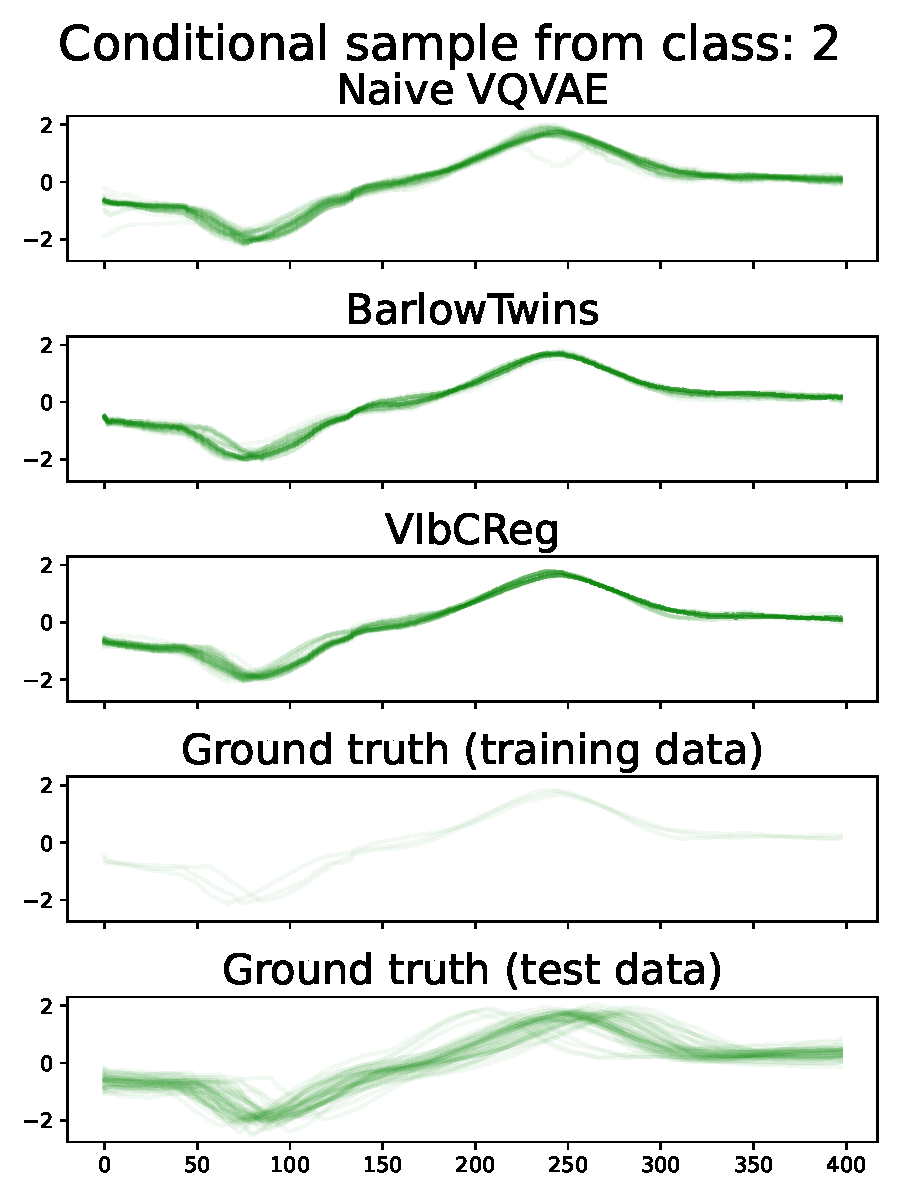
\includegraphics[width=\textwidth]{Symbols-conditional-class2.pdf}
    \end{minipage}
    % \hfill
    \begin{minipage}[b]{0.32\textwidth}
        \centering
        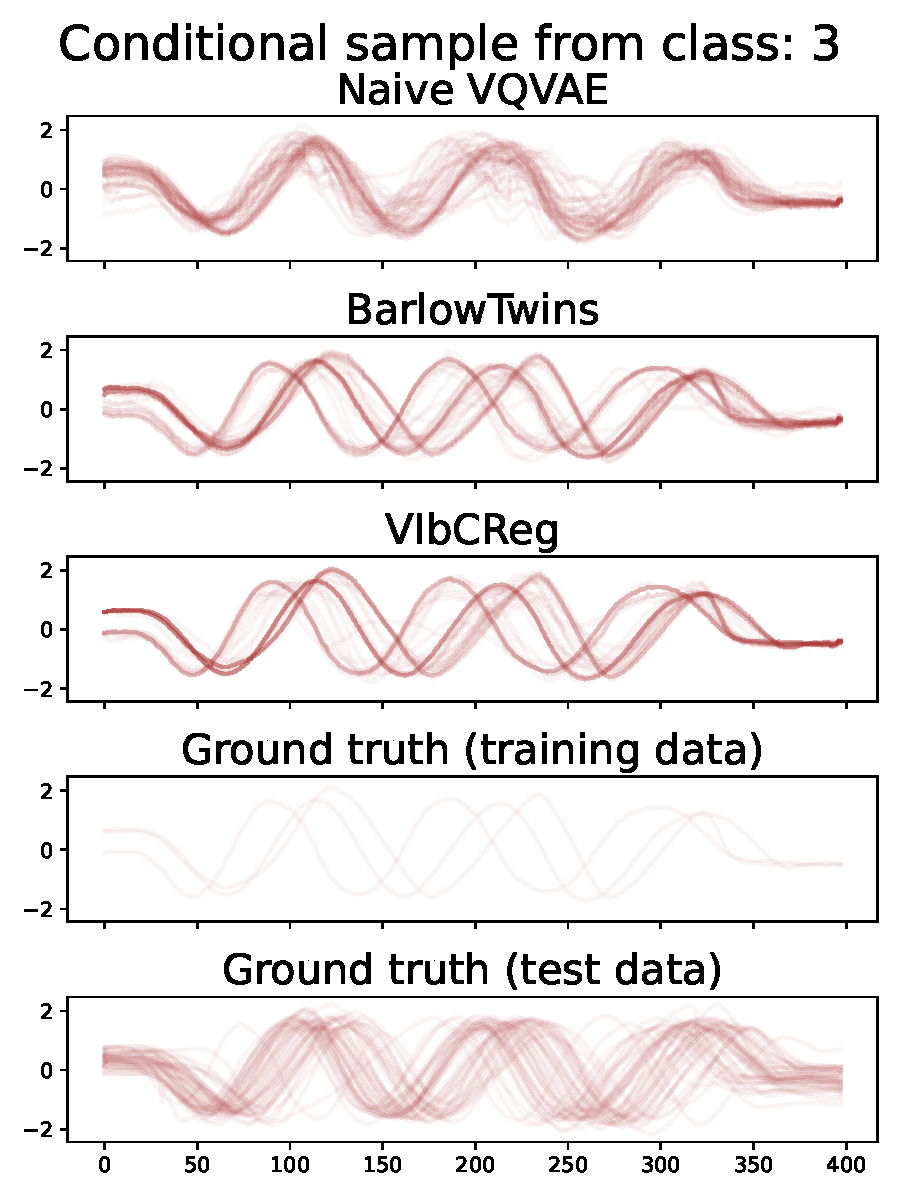
\includegraphics[width=\textwidth]{Symbols-conditional-class3.pdf}
    \end{minipage}
    \begin{minipage}[b]{0.32\textwidth}
        \centering
        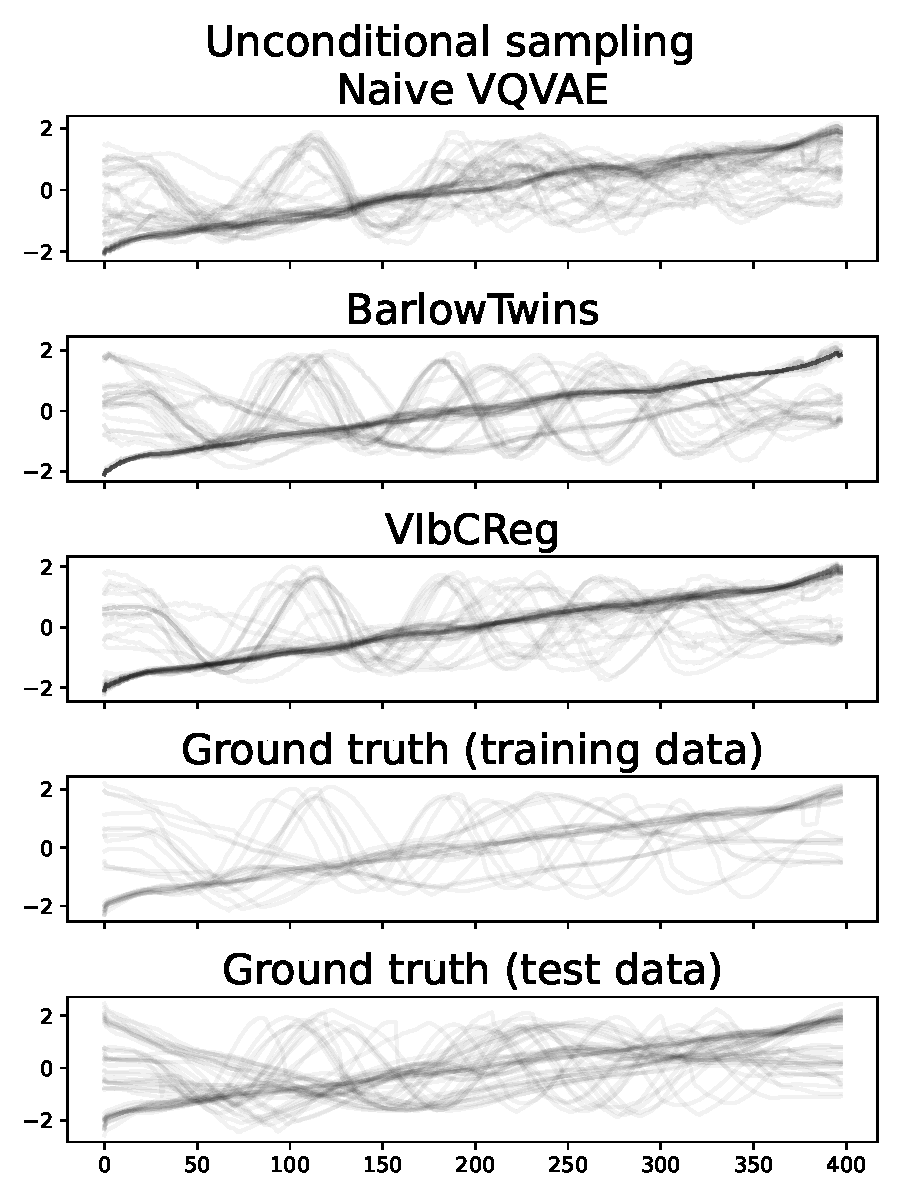
\includegraphics[width=\textwidth]{Symbols-unconditional.pdf}
    \end{minipage}
    \caption{Class conditional distribution for some selected classes of Symbols. Barlow and VIbCReg both trained with gaussian augmentation.}
    \label{fig:Gauss_Symbols}
\end{figure}






\subsubsection{ShapesALL}
The dataset ShapesAll consists of 60 classes, with 10 samples within each class. Each class has distinct patterns, with varying complexity.\newline

In Figure \ref{fig:Gauss_ShapesAll}, we observe clearly that naive VQVAE struggles with capturing the global consistency of the samples. We too observe that Barlow Twins mimic the training slightly more closely than VIbCReg, which provides some insight as to why Barlow Twins improves CAS by about 10 percent compared to naive VQVAE. Both Barlow Twins and VIbCReg improve IS, but fail to improve FID. As we have seen in the other datasets with few samples for a specific class, NC-VQVAE has a tendency to overfit.

\begin{figure}[H]
    \centering
    \begin{minipage}[b]{0.32\textwidth}
        \centering
        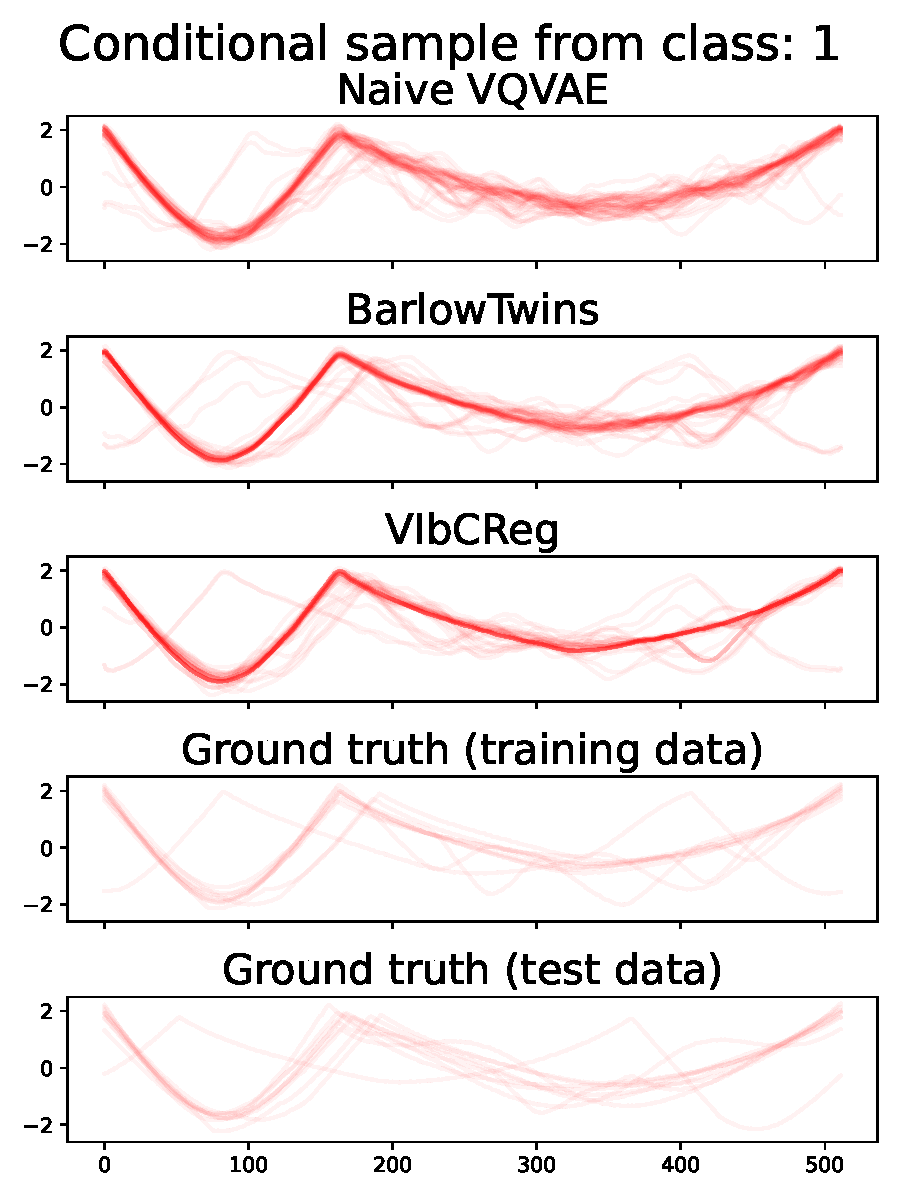
\includegraphics[width=\textwidth]{ShapesAll-conditional-class1.pdf}
    \end{minipage}
    % \hfill
    \begin{minipage}[b]{0.32\textwidth}
        \centering
        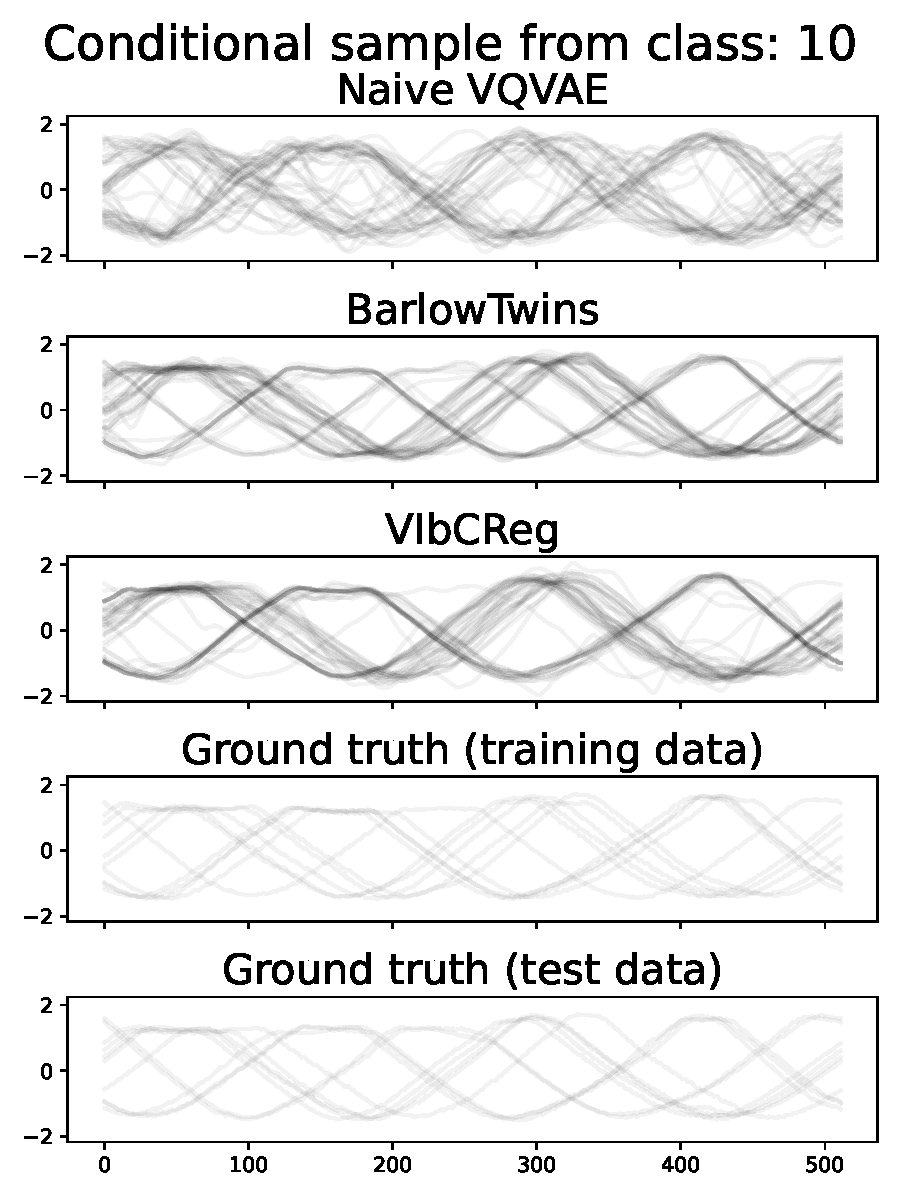
\includegraphics[width=\textwidth]{ShapesAll-conditional-class10.pdf}
    \end{minipage}
    \begin{minipage}[b]{0.32\textwidth}
        \centering
        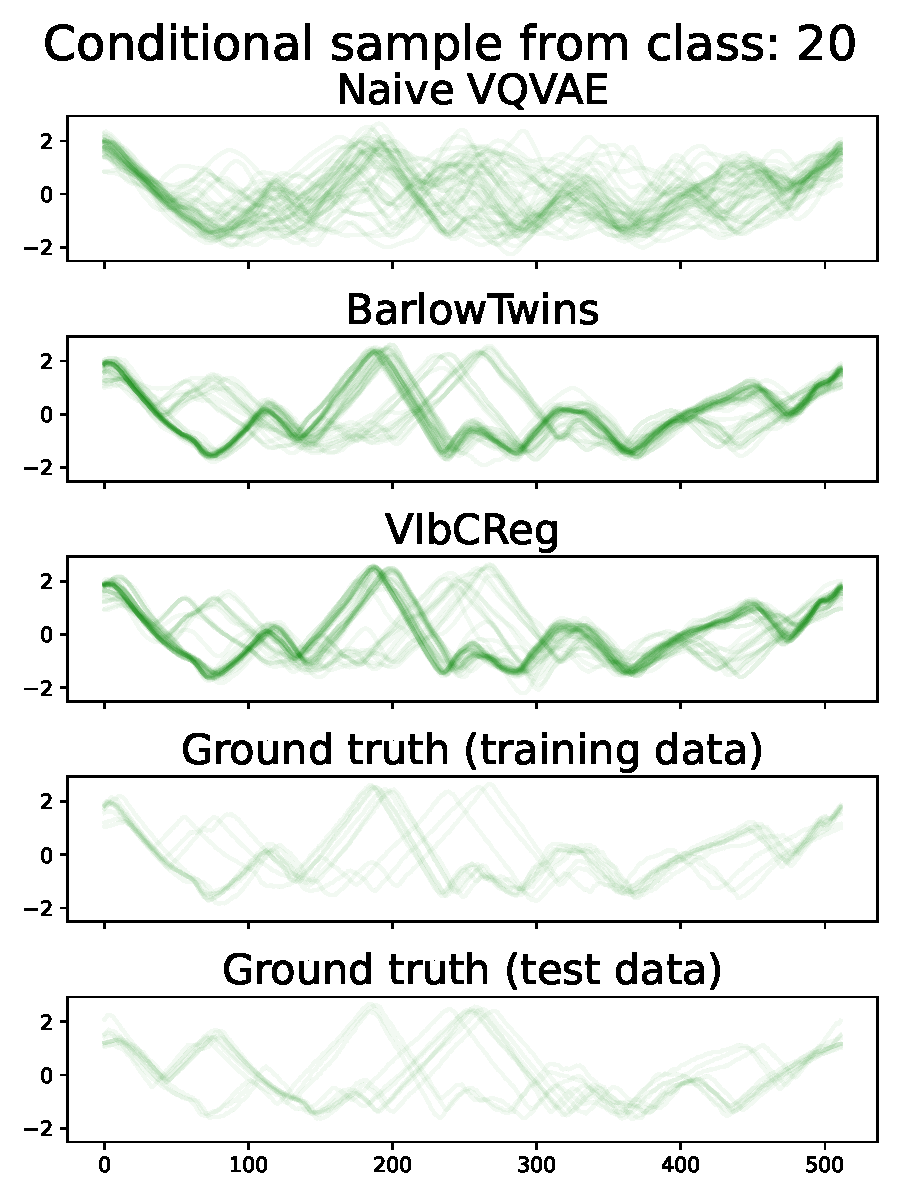
\includegraphics[width=\textwidth]{ShapesAll-conditional-class20.pdf}
    \end{minipage}
    \caption{Class conditional distribution for some selected classes of ShapesAll. Barlow and VIbCReg both trained with gaussian augmentation.}
    \label{fig:Gauss_ShapesAll}
\end{figure}



\subsubsection{UWaveGestureLibraryAll}
The dataset UWaveGestureLibraryAll contains time series with distinct discontinuities and sharp changes in modularity. As noted in \cite{TimeVQVAE}, such datasets are challenging to model.\newline

In Figure \ref{fig:Warp_Uwave} a selected subset of classes are illustrated. We observe upon close inspection that VIbCReg maintains variability in the samples to a greater degree than Barlow Twins, as well at slightly better capturing the "dead spots" following the discontinuities. \newline 


\begin{figure}[H]
    \centering
    % \hfill
    \begin{minipage}[b]{0.32\textwidth}
        \centering
        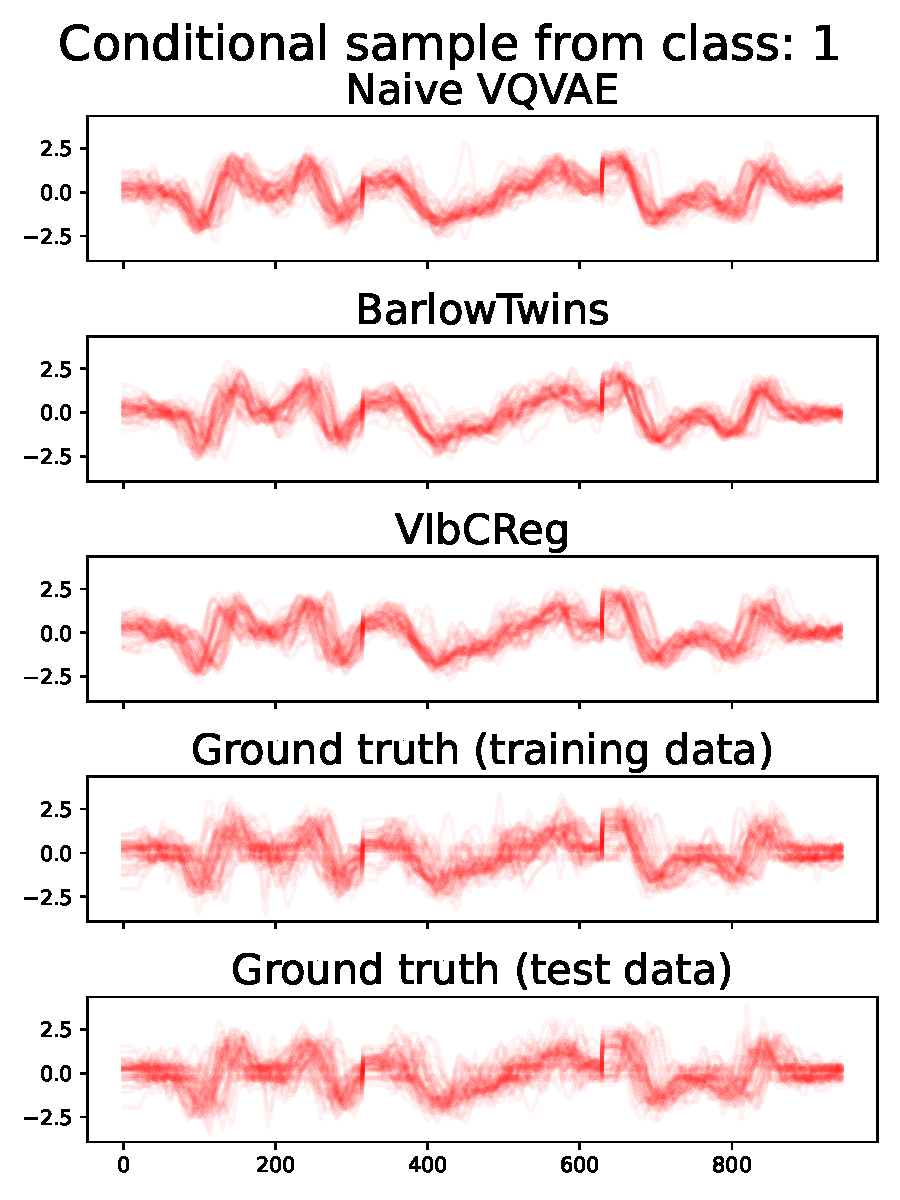
\includegraphics[width=\textwidth]{UWaveGestureLibraryAll-conditional-class1.pdf}
    \end{minipage}
    \begin{minipage}[b]{0.32\textwidth}
        \centering
        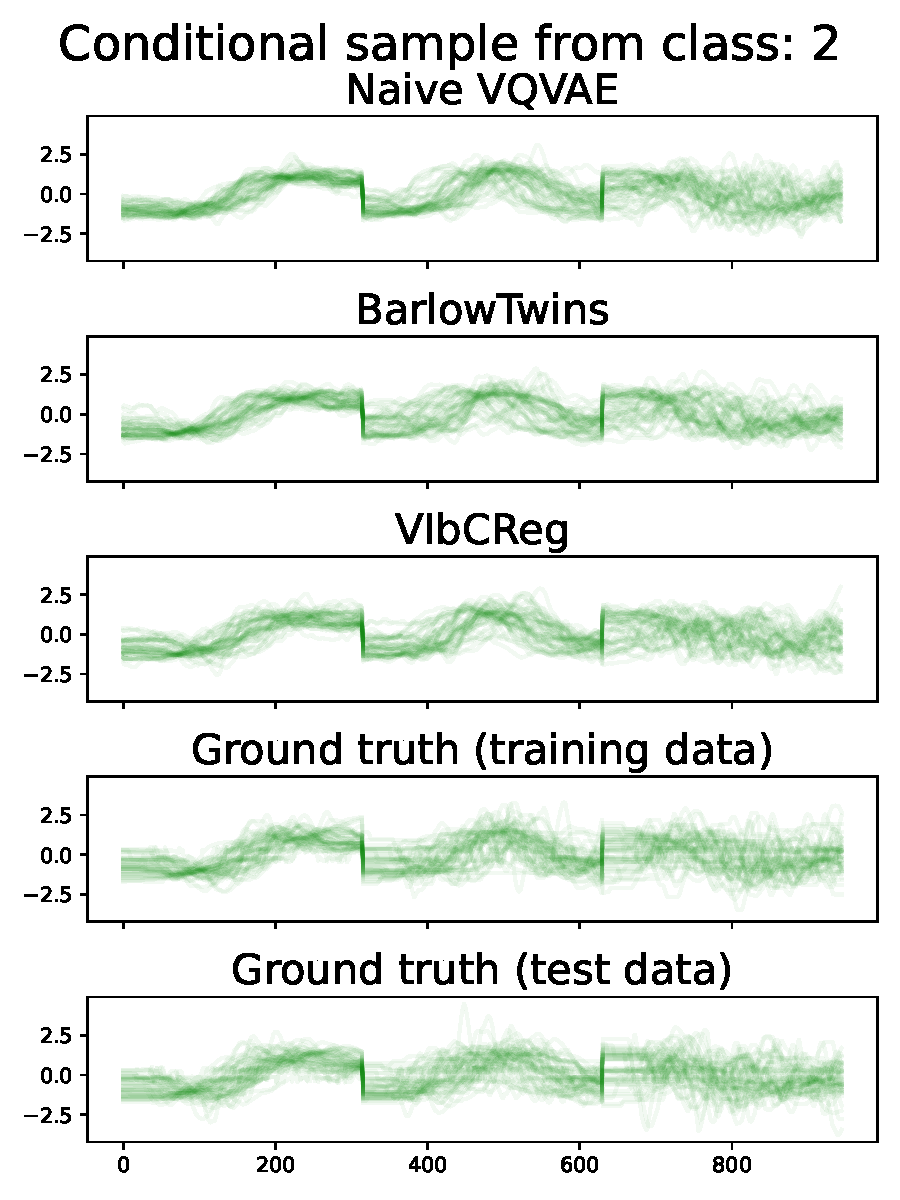
\includegraphics[width=\textwidth]{UWaveGestureLibraryAll-conditional-class2.pdf}
    \end{minipage}
    \begin{minipage}[b]{0.32\textwidth}
        \centering
        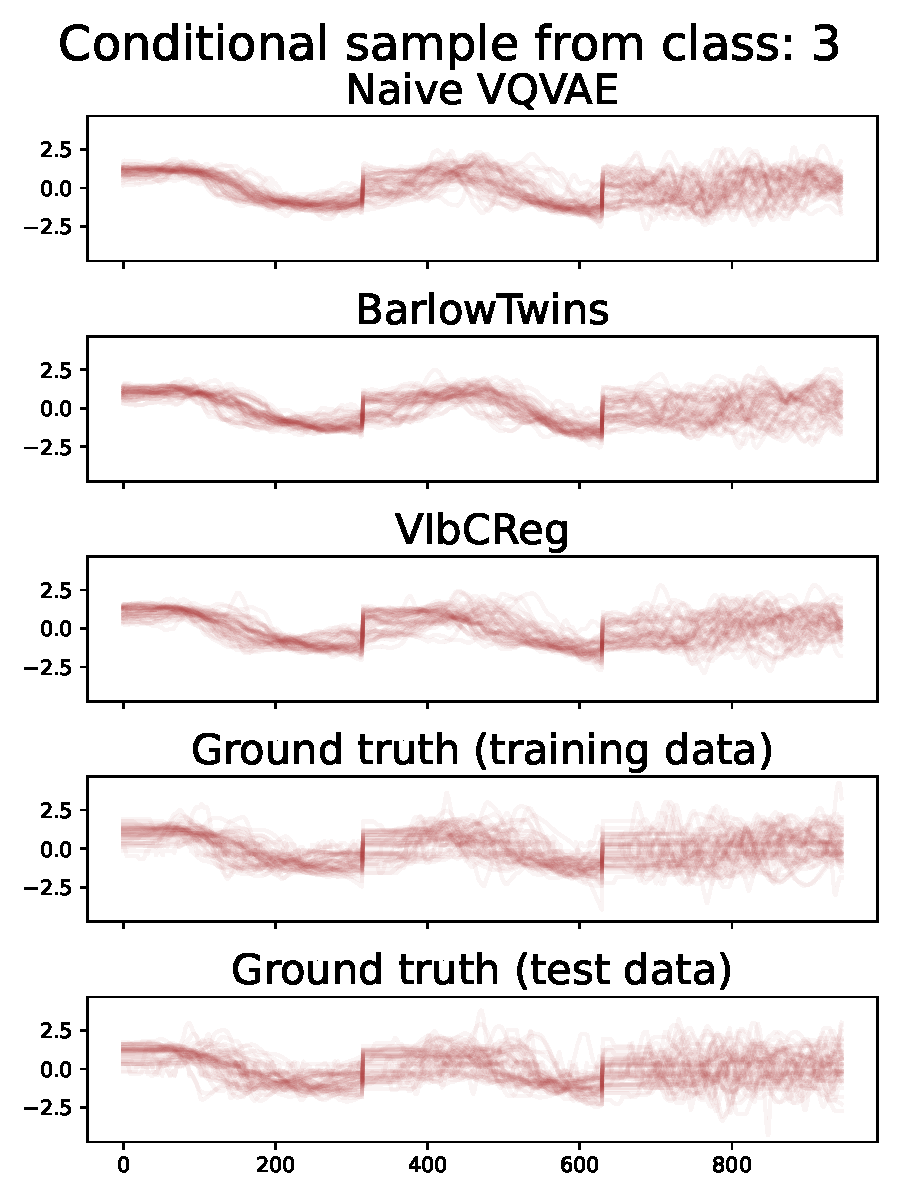
\includegraphics[width=\textwidth]{UWaveGestureLibraryAll-conditional-class3.pdf}
    \end{minipage}
    \caption{Class conditional distribution for some selected classes of UWaveGestureLibraryAll. Barlow and VIbCReg both trained with window warp and amplitude resize augmentations.}
    \label{fig:Warp_Uwave}
\end{figure}






\section{Differences in Barlow Twins and VIbCReg}

VIbCReg seems to keep the variability in the conditional distribution a bit better than Barlow Twins. Can it be attributed to the variance term in VIbCReg?

\begin{figure}[H]
    \centering
    % \hfill
    \begin{minipage}[b]{0.48\textwidth}
        \centering
        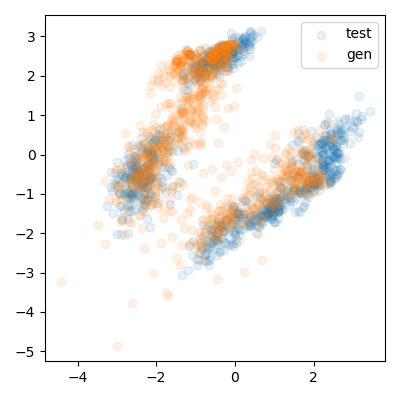
\includegraphics[width=\textwidth]{VIB_gauss_latentspace_PCA_Mallat.png}
    \end{minipage}
    \begin{minipage}[b]{0.48\textwidth}
        \centering
        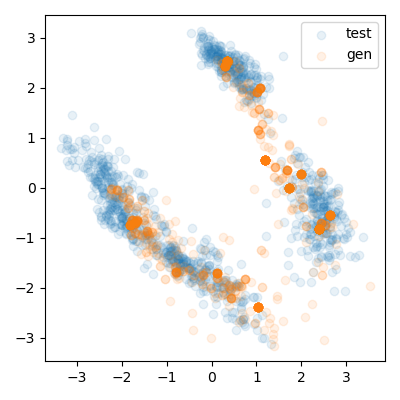
\includegraphics[width=\textwidth]{BT_gauss_latentspace_PCA_Mallat.png}
    \end{minipage}
    \caption{PCA of discrete latent representation from Mallat. Both VIbCReg (left) and Barlow Twins (right) are trained with gaussian augmentation.}
    \label{fig:Mallat_latent_PCA}
\end{figure}

\begin{figure}[H]
    \centering
    % \hfill
    \begin{minipage}[b]{0.48\textwidth}
        \centering
        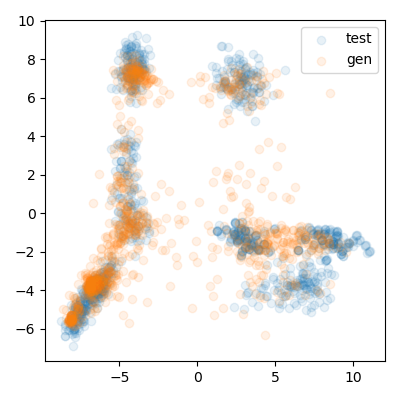
\includegraphics[width=\textwidth]{VIB_gauss_dataspace_PCA_Mallat.png}
    \end{minipage}
    \begin{minipage}[b]{0.48\textwidth}
        \centering
        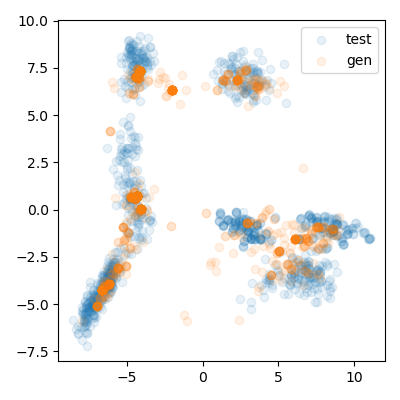
\includegraphics[width=\textwidth]{BT_gauss_dataspace_PCA_Mallat.png}
    \end{minipage}
    \caption{PCA of generated time series from Mallat. Both VIbCReg (left) and Barlow Twins (right) are trained with gaussian augmentation.}
    \label{fig:Mallat_data_PCA}
\end{figure}


\subsection{Overfitting problem}

We have observed on multiple occasions that when the sample size is small and the patterns in the data are simple NC-VQVAE has a tendency to overfit, and memorize the training data to a large degree. We have not employed any form of dropout or other regularization techniques when training on small datasets. 

\subsection{Thoughts}

Better inception score and CAS of our models indicate that the class separability learned in latent space makes the conditional distributions more distinct easier to classify. The FID is variable, but in many cases better, which indicated that the generative distributions are closer to the ground truth.\newline

Gaussian noise aug seems to result in a lot easier the BT/VIbCReg loss to minimize. \newline
Slice and shuffle is harder to minimize, but could seem to push representations for different classes further apart resulting in better linear probes.\newline

Talk about the difficulty/ease in minimizing the SSL loss for the different augmentations. Does this affect linear probes / reconstruction / FID / IS / Prior loss
\newline



For datasets of smaller size with classes of different characteristics (a clear distributional difference in visual inspection [Sony2 and Symbols]) NC-VQVAE seems to perform better both in terms of FID and IS. \newline

The biases introduced by augmentations in stage 1 seems to be included in the generated samples to some degree. In particular datasets with high frequency components, when applying Gaussian noise (easier to spot), has substantially better FID score.  \newline

Is there correlation between CAS and linear probe accuracy?? \newline

Temporal vs frequency influence of augmentations. We compress only along temporal axis in the encoder. Could this be a reason for Gaussian artifacts in generation and not slice?\newline


\subsection{Augmentation Reconstruction Weight}
\begin{figure}[h]
    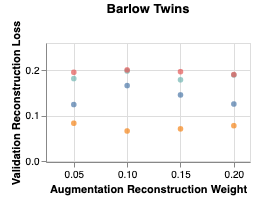
\includegraphics[scale=0.55]{BT_ValRecons_ReconsWeight.png}
    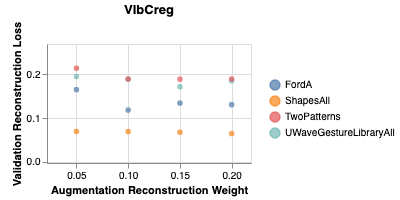
\includegraphics[scale=0.55]{ViB_ValRecons_ReconsWeight.png}
    % \centering  
    \caption{Augmentation: Window Warp and Amplitude Resize. Averaged across 2 runs. Trained for 250 epochs}  
    \label{fig:ReconsWeight_warp}
\end{figure}
\begin{figure}[h]
    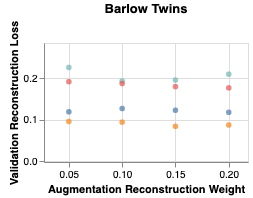
\includegraphics[scale=0.55]{BT_ValRecons_ReconsWeight_Slice.png}
    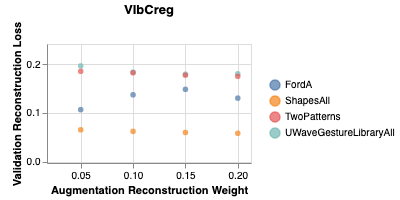
\includegraphics[scale=0.55]{ViB_ValRecons_ReconsWeight_Slice.png}
    % \centering  
    \caption{Augmentation: Slice and Shuffle. Averaged across 2 runs. Trained for 250 epochs}  
    \label{fig:ReconsWeight_slice}
\end{figure}


% \subsection{Augmentation Reconstruction Weight}
% Here are the results of the ablation on the effect of “Augmentation Reconstruction Weight” on Stage 1.
% “Augmentation Reconstruction Weight” is the weight given to the reconstruction loss on the augmented branch.
% Tested weights $0.05$, $0.1$, $0.15$ and $0.2$.
% Augmentations [Window Warp, Amplitude Resize] and [Slice and Shuffle].
% The weight has little effect on linear probe accuracy across the four datasets tested, and the two sets of augmentations.
% The effect on Validation reconstruction loss is small for all except FordA.
% It seems, not very surprisingly, that the choice of augmentations are of (much) greater importance.
% \begin{figure}[h]
%     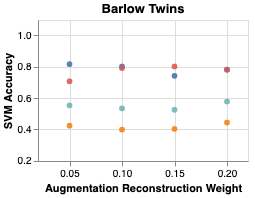
\includegraphics[scale=0.55]{BT_SVM_ReconsWeight.png}
%     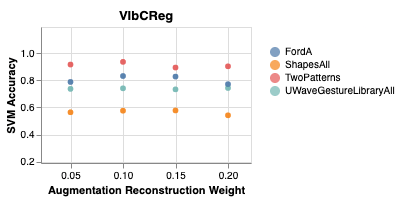
\includegraphics[scale=0.55]{ViB_SVM_ReconsWeight.png}
%     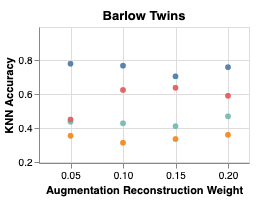
\includegraphics[scale=0.55]{BT_KNN_ReconsWeight.png}
%     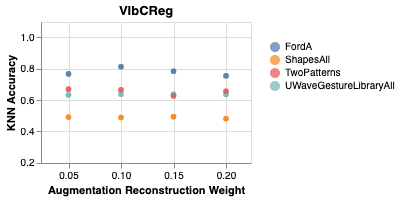
\includegraphics[scale=0.55]{ViB_KNN_ReconsWeight.png}
%     \centering  
%     \caption{Augmentations: Window Warp and amplitude resize. Averaged across 2 runs. Trained for 250 epochs}  
% \end{figure}

% \begin{figure}[h]
%     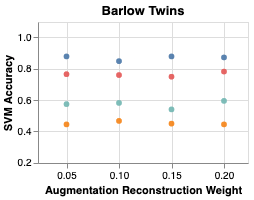
\includegraphics[scale=0.55]{BT_SVM_ReconsWeight_Slice.png}
%     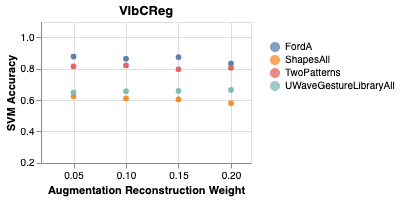
\includegraphics[scale=0.55]{ViB_SVM_ReconsWeight_Slice.png}
%     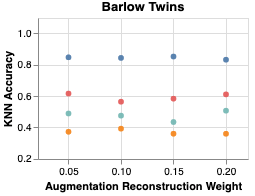
\includegraphics[scale=0.55]{BT_KNN_ReconsWeight_Slice.png}
%     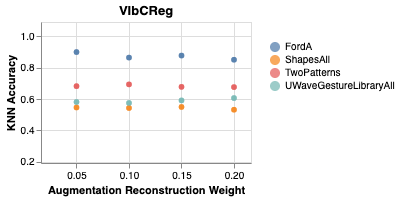
\includegraphics[scale=0.55]{ViB_KNN_ReconsWeight_Slice.png}

%     % \centering  
%     \caption{Augmentation: Slice and shuffle. Averaged across 2 runs. Trained for 250 epochs}  
% \end{figure}

% \begin{figure}[h]
%     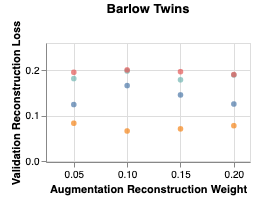
\includegraphics[scale=0.55]{BT_ValRecons_ReconsWeight.png}
%     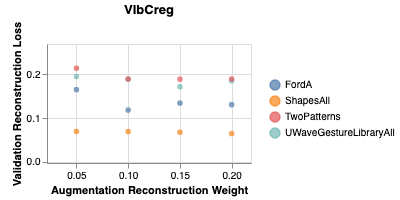
\includegraphics[scale=0.55]{ViB_ValRecons_ReconsWeight.png}
%     % \centering  
%     \caption{Augmentation: Window Warp and amplitude resize. Averaged across 2 runs. Trained for 250 epochs}  
% \end{figure}
% \begin{figure}[h]
%     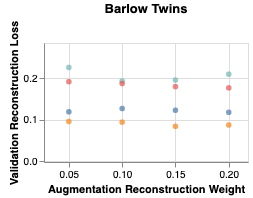
\includegraphics[scale=0.55]{BT_ValRecons_ReconsWeight_Slice.png}
%     \includegraphics[scale=0.55]{ViB_ValRecons_ReconsWeight_Slice.png}
%     % \centering  
%     \caption{Augmentation: Slice and shuffle. Averaged across 2 runs. Trained for 250 epochs}  
% \end{figure}
% \subsection{Augmentation robustness}
% \label{section:Augmentation robustness}
% S1 - S2 - Augs: Choose datasets such that half were thought to be well fitting for slice and shuffle and half for amplitude resize + window Warp. This was after seeing FordA performing well with S and S, and looking at the augmented views.\newline
% FordA/B, Electric devices, ShapesALL for S and S\newline
% TwoP, UWave, symbols, Mallat for ampRes + winwarp\newline

% Visual inspection: Plot training samples + spectrogram, compare to augmented view. Compare these against others from other classes. \newline
% Does the resulting improvement in stage 1 transfer to stage 2? 

% \TODO{Download the Wandb data.}
% Plot for each dataset and each augmentation: 
% Color code according to SSL-model.


\section{Conclusion}
Even though there are issues, we believe our model is a step in the right direction. The representations learned by NC-VQVAE are more expressive than naive VQVAE, demonstrating that we can optimize more than one objective, without sacrificing the reconstruction capability. 

The representations enable easier learning of the semantics of the conditional distributions, to such a degree that one has to take measures not to overfit. 

The representations makes it easier to capture the gobal consistency of the samples, which tha naive VQVAE has large issues with. This without the HF-LF split.

The added flexibility of NC-VQVAE, with possibility of choosing dataset specific augmentations, can in some applications be beneficial.\newline


\section{Further work}



\cite{morningstar2024augmentations} suggest that focus on augmentations is of great importance. The hunt for good augmentations in the time series domain is ongoing and should probably get more attention.\newline
HF-LF split - augmentations tailored for HF and LF, as they often have quite different characteristics.\newline
Wavelet transform to improve HF-LF split.\newline

Further optimize the relationship between aug recon loss and choice of augmentations.\newline

Improving on the stage 2 learning to better handle the expressive representations, and be able to create more diverse samples. Higher masking ratio during training, lower value for $T$ etc.\newline

The differences in Barlow and VIbCReg indicate that further optimization of the SSL method/pretext task for generative performance is possible and could be an interesting extension of this project. \newline

Investigation of the attention maps. Could one find if there is a HF direction, translation direction etc. similarly to how one in NLP can find gender direction, nationality direction etc?






\end{document}